\chapter{Experimental Apparatus}
\label{chap:Exp}

\indent The study of standard model (SM) physics at the TeV scale and search for potentially new physics beyond the standard model (BSM) is one of the highlights of current physics programs at the Large Hadron Collider (LHC).  The LHC is a circular superconducting particle accelerator capable of accelerating and colliding both protons and lead ions.  The LHC is built in the 27km LEP tunnel between 45 to 170m underground near the city of Geneva.  The entire LHC accelerator complex, shown in Figure \ref{LHC:fig:LHCComplex} is operated by the Organization for European Nuclear Research or CERN. More details on the LHC machine and the CERN accelerator complex can be found in reference [\cite{LHC}]. \\

\begin{figure}[h!]
%\begin{center}
\centering
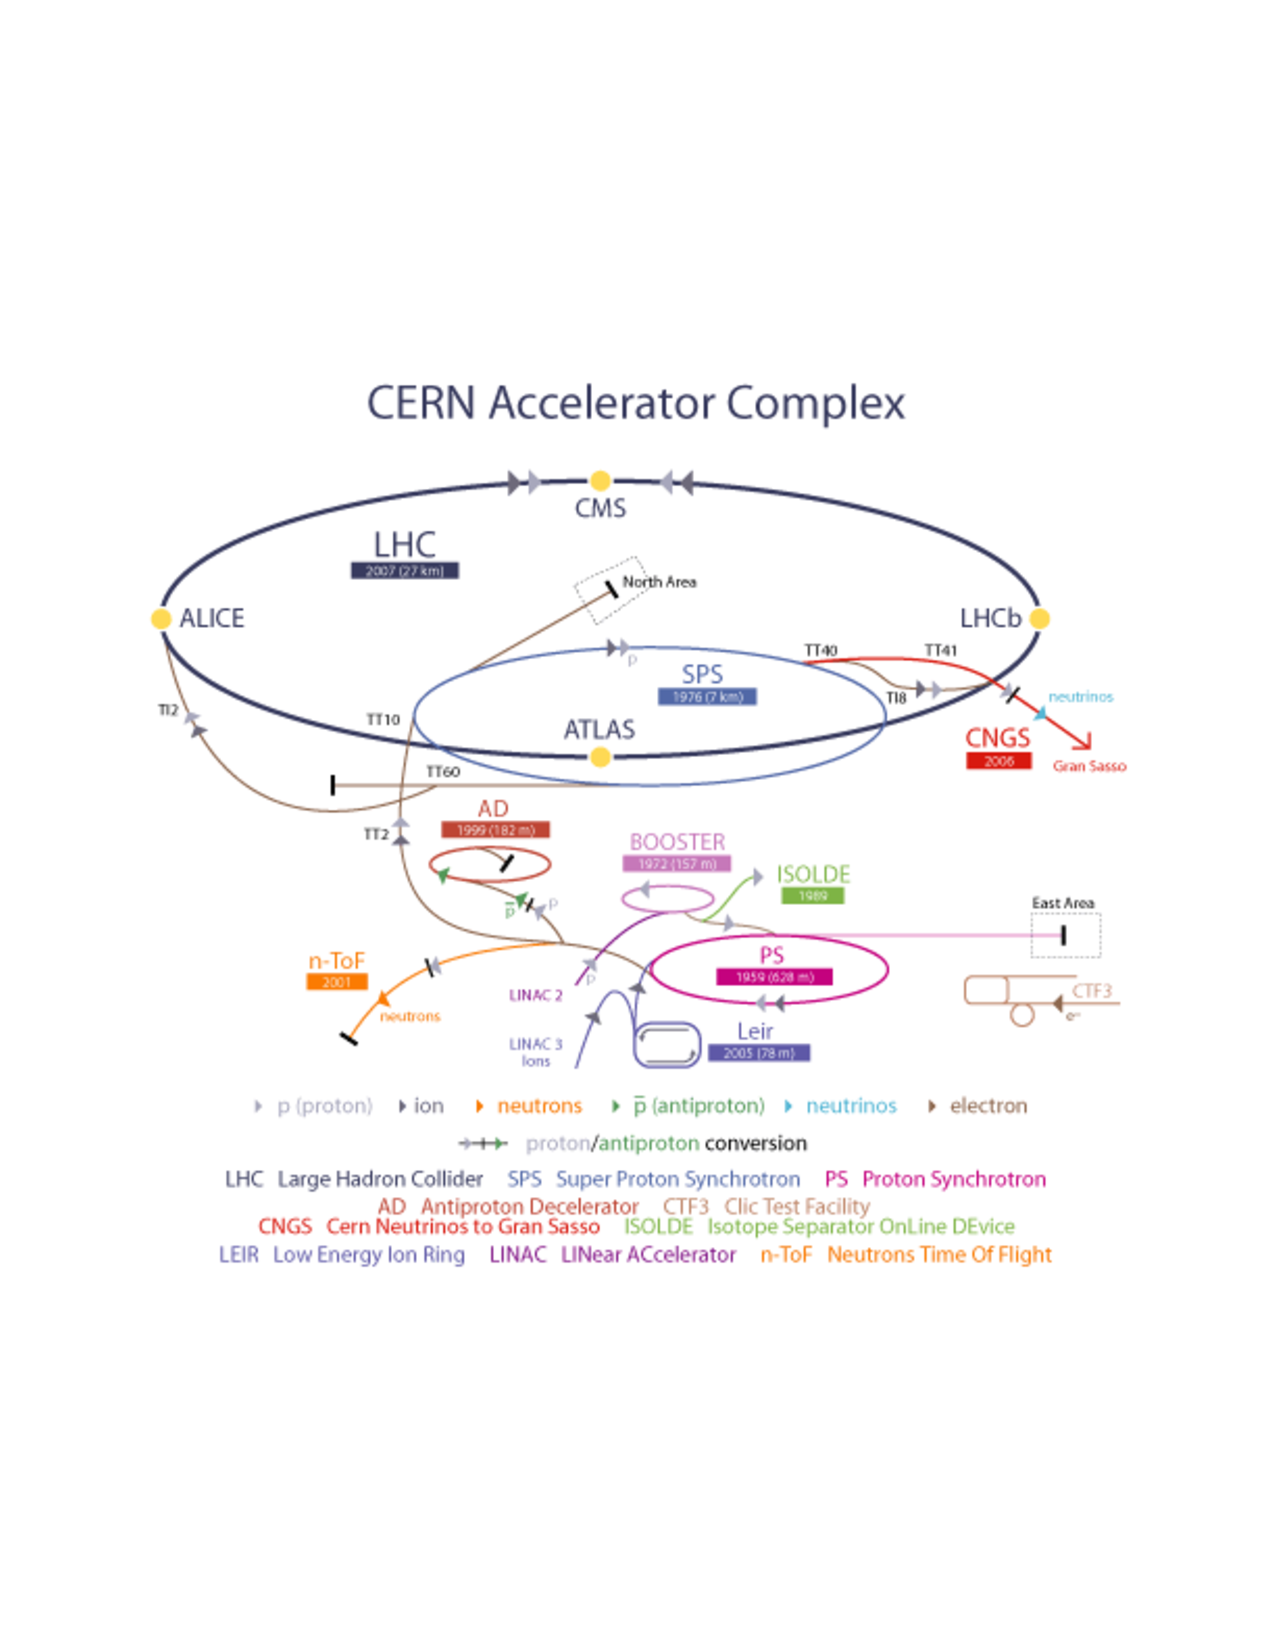
\includegraphics[width=0.95\textwidth, angle=0]{figures/LHC_ATLAS/AccComplex0700829.pdf}
\caption{ The Large Hadron Collider complex.\cite{LHC} \label{LHC:fig:LHCComplex}}
%\end{center}
\end{figure}

\indent During 2015 to 2016, the LHC collided protons with a center of mass energy of $13$ TeV.  During 2016, the LHC surpassed its design by reaching peak instantaneous luminosities of $1.34 \times 10^{34}$ cm$^{-2}$ sec$^{-1}$.  \\

\indent The LHC uses four major particle detectors located at four interaction points at different locations in the ring to study the result of these collisions.  Two of these, ATLAS and CMS, are hermetic  $4\pi$ general-purpose detectors that study a wide variety of SM and BSM physics including SUSY.   ATLAS and CMS are located at the opposite ends of the ring to ensure equal integrated luminosity.  The two detectors are sensitive to the same physics processes and serve as validations to one another.  The ALICE detector specializes in the collision of heavy ions and LHCb specializes in physics involving the bottom quark. \\

\indent In addition to the 4 major particle detectors, three smaller experiments, TOTEM, MoEDAL and LHCf, study proton-proton scattering cross sections, diffractive processes, and cosmic ray physics.  ~\\

\indent This analysis uses data collected by the ATLAS detector in 2015 and 2016.  A summary of the ATLAS detector is given in section \ref{LHC:detector}. \\

%\section{The CERN Accelerator Complex and the Large Hadron Collider}

%\indent Before collision in one of the LHC experiments, protons are first accelerated through a series of accelerators that form the CERN accelerator complex shown in Figure \ref{LHC:fig:LHCComplex}.  Hydrogen atoms are ionized and the resulting protons are first accelerated to $50 \mev$ by the Linear Accelerator 2 (LINAC2).  Then the protons are injected into a series of circular accelerators, the Proton Synchrotron Booster (PSB), the Proton Synchrotron (PS) and Super Proton Synchrotron (SPS) that further increases the proton energy to 1.4, 25 and 450 GeV respectively.  The protons are arranged into bunches composed of approximately $1.1 \times 10^{11}$ protons each and injected into the LHC.  During 2015 and 2016, the LHC operated with both 50 ns and 25 bunch spacings and can nominally accommodate up to 2808 bunches in a single run. \\

%\begin{figure}[h!]
%\begin{center}
%\centering
%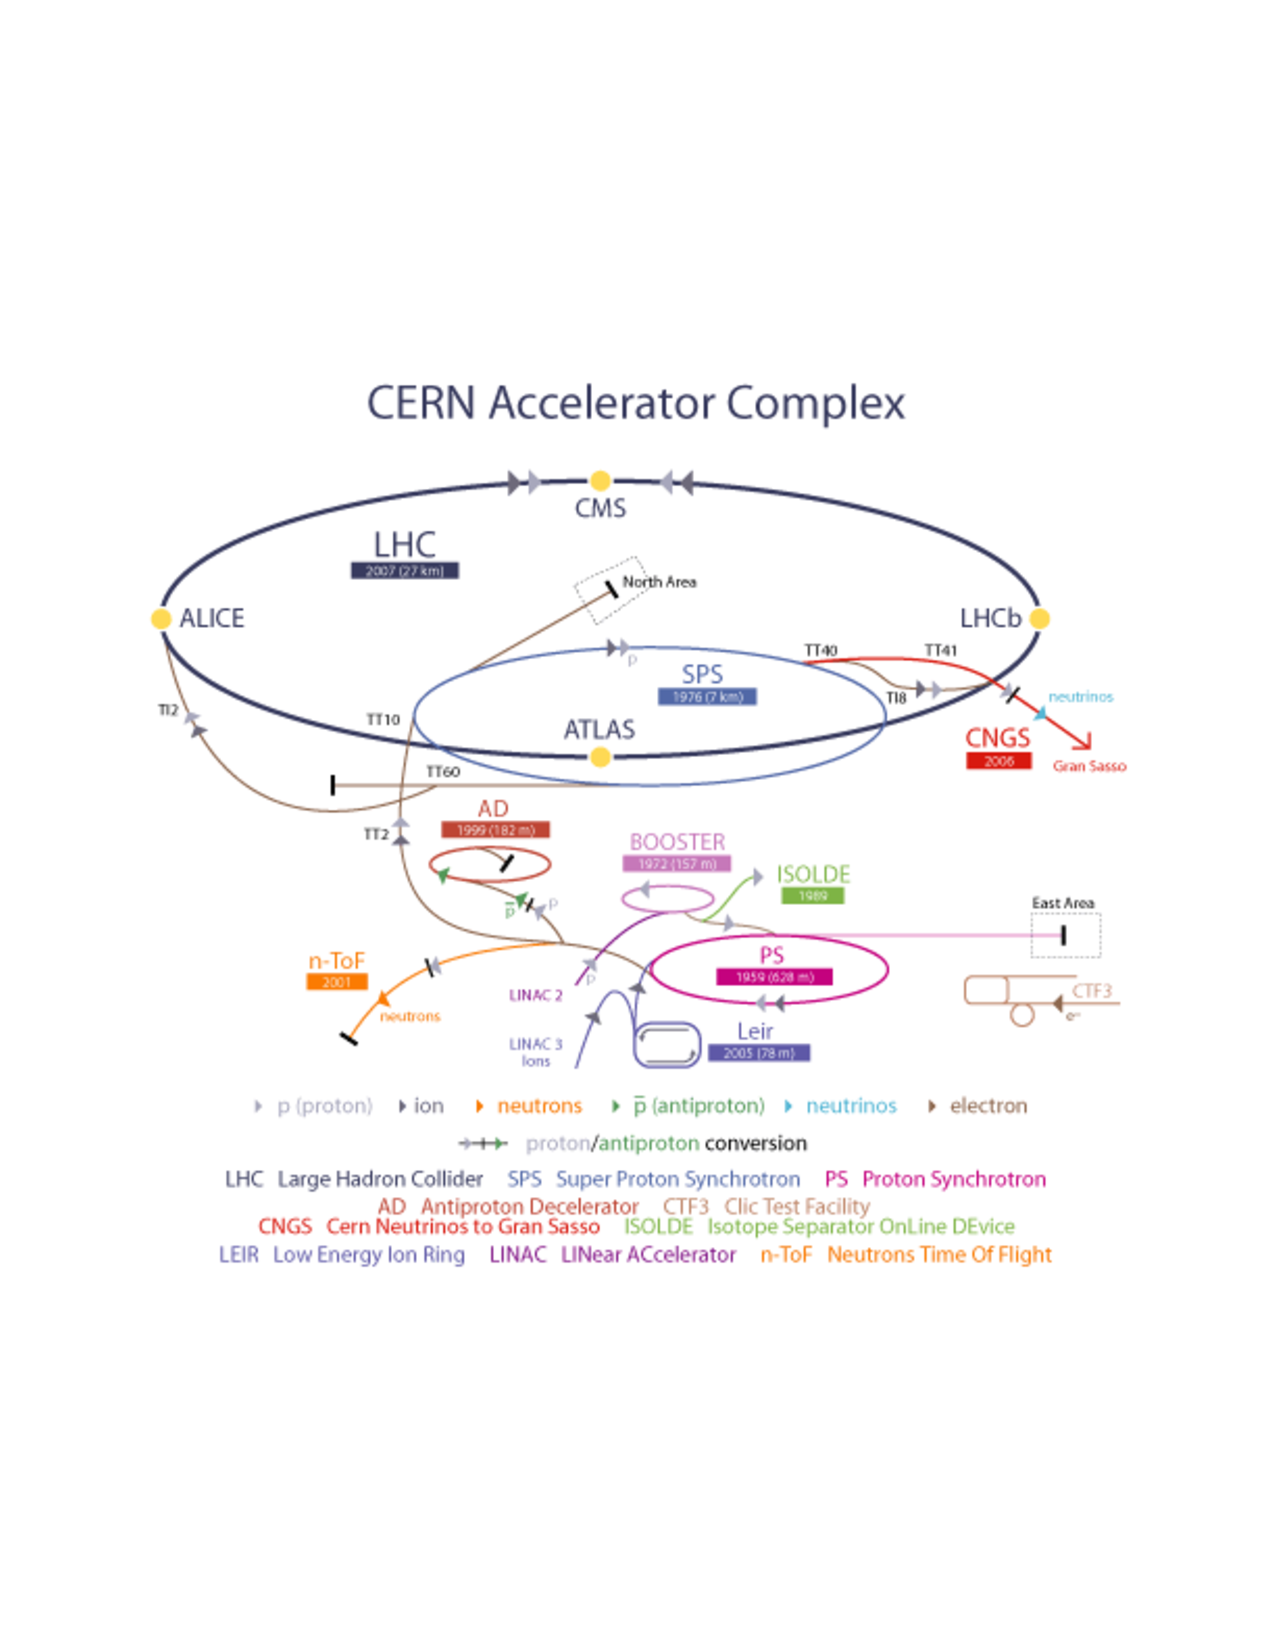
\includegraphics[width=0.65\textwidth, angle=0]{figures/LHC_ATLAS/AccComplex0700829.pdf}
%\caption{ The Large Hadron Collider complex. (Taken from \cite{LHC}) \label{LHC:fig:LHCComplex}}
%\end{center}
%\end{figure}

%\indent The LHC shares the same geometry as LEP with eight arc and eight straight sections.  The main LHC body consist of 1232 dipole Niobium Titanium superconducting magnets that are used to generate the 8.33 Tesla magnetic field necessary to bend the 7 TeV proton beams.  The LHC uses a {\tt two-in-one} magnet design shown in figure \ref{LHC_Xsec} both as a cost saving measure and because of the limited space in the tunnels. The two-in-one magnet design uses a single cryogenic system and vacuum vessel for both proton beams.  \\

%\begin{figure}[h!]
%\begin{center}
%\centering
%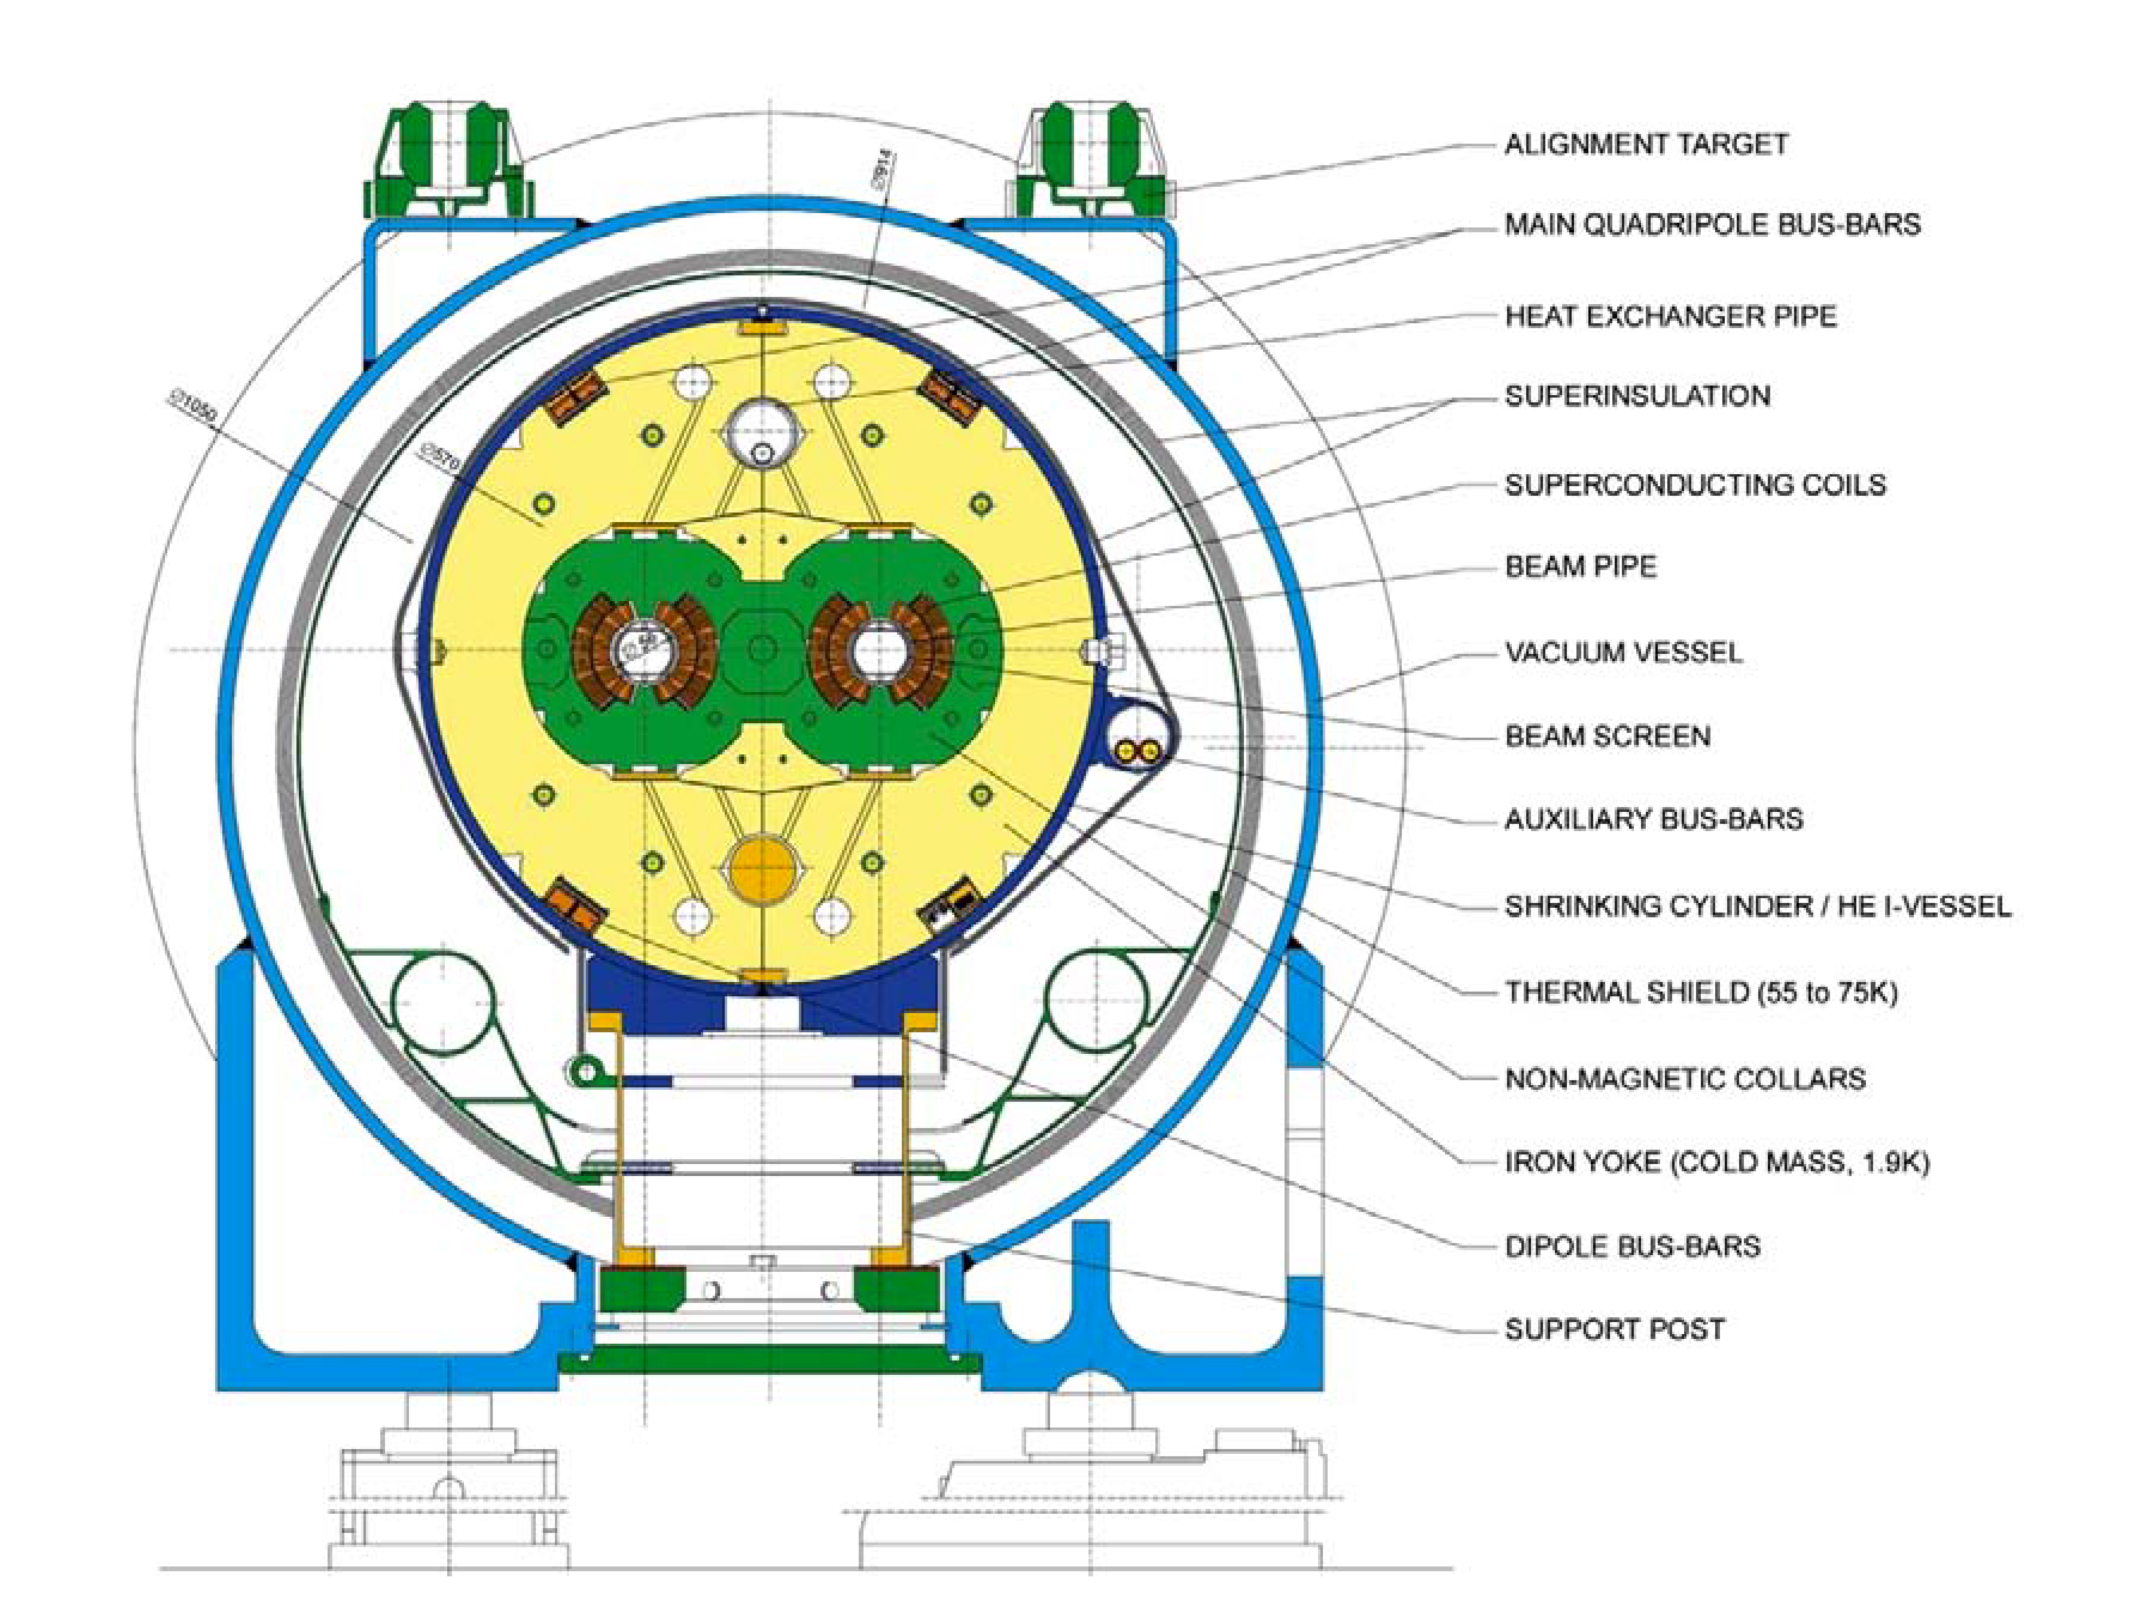
\includegraphics[width=0.75\textwidth]{figures/LHC_ATLAS/LHCCrossSection.pdf}
%\caption{ Cross-Sectional View of a Large Hadron Collider Dipole Magnet.\cite{LHC} }
%\label{LHC_Xsec}
%\end{center}
%\end{figure}

%\indent  392 quadruple magnets are placed after approximately every three dipole sections to stabilize and focus the beam using the principle of strong focusing.  Higher order sextupoles and octupoles magnets provide further corrections. \\

%\indent The beams are accelerated using a 400 MHz superconducting radio frequency (RF) cavity system.  Two independent RF systems are used for the two beams heading in opposite directions.  Each RF system consists of eight cavities.  The total accelerating field inside the cavity is 5 MV/m and each cavity delivers 2 MV of accelerating voltage.  The beams are bent back to repeatedly receive acceleration via the same cavity.  \\

%\indent Further upgrades planed in the Phase 1 shutdown between 2019 and 2021 are projected to further double the instantaneous luminosity and allow the LHC to reach its designed center of mass collision energy of $\sqrt{14} \tev$. \cite{Phase1} \\

\section{The ATLAS Detector}
\label{LHC:detector}

\indent The ATLAS Detector is a general purpose detector designed to search for new physics at the TeV scale and precisely measure SM parameters.  The ATLAS detector is composed of several subdetectors arranged in concentric cylinders surrounding the interaction point.  The hermetic detector covers nearly the entire $4\pi$ solid angle around the interaction point. A cutaway view of the ATLAS detector can be seen in Figure \ref{LHC:fig:ATLASDet}.  For more details on the ATLAS detector design and specifications see reference [\cite{ATLAS_JINST}].  \\

%define coordinate system.  Phi, eta, Z

\begin{figure}[h!]
%\begin{center}
\centering
\includegraphics[width=0.85\textwidth, angle=0]{figures/LHC_ATLAS/ATLAS_SE_Corrected7.eps}
\caption{ Cutaway view of the ATLAS detector with different sub-detector systems labeled. \label{LHC:fig:ATLASDet}}
%\end{center}
\end{figure}

\indent A coordinate system is defined with the nominal interaction point as the origin.  The x-axis points to the center of the LHC ring and the y-axis points upwards.  The z-axis points along the beam line.  The A-side of the detector is defined to be the half with positive z and the C-side of the detector is the half with negative z.  The azimuthal angle $\phi$ is defined to be around the beam axis in the x-y plane and the polar angle $\theta$ is defined to be from the z-axis.  The pseudorapidity, $\eta = -\ln  \tan (\theta/2) $, is often used instead of the coordinate $\theta$.  \\%In the case of massive objects, the rapidity, $\gamma = 1/2 \ln[( E+p_z )( E-p_z )]$ is also used instead. \\

\indent The detector can be divided into the inner detector, the electromagnetic calorimeter, the hadronic calorimeter and the muon spectrometer.  The detector signatures left by different particles can be seen in Figure \ref{LHC:fig:ATLASSig}. \\

\begin{figure}[h!]
%\begin{center}
\centering
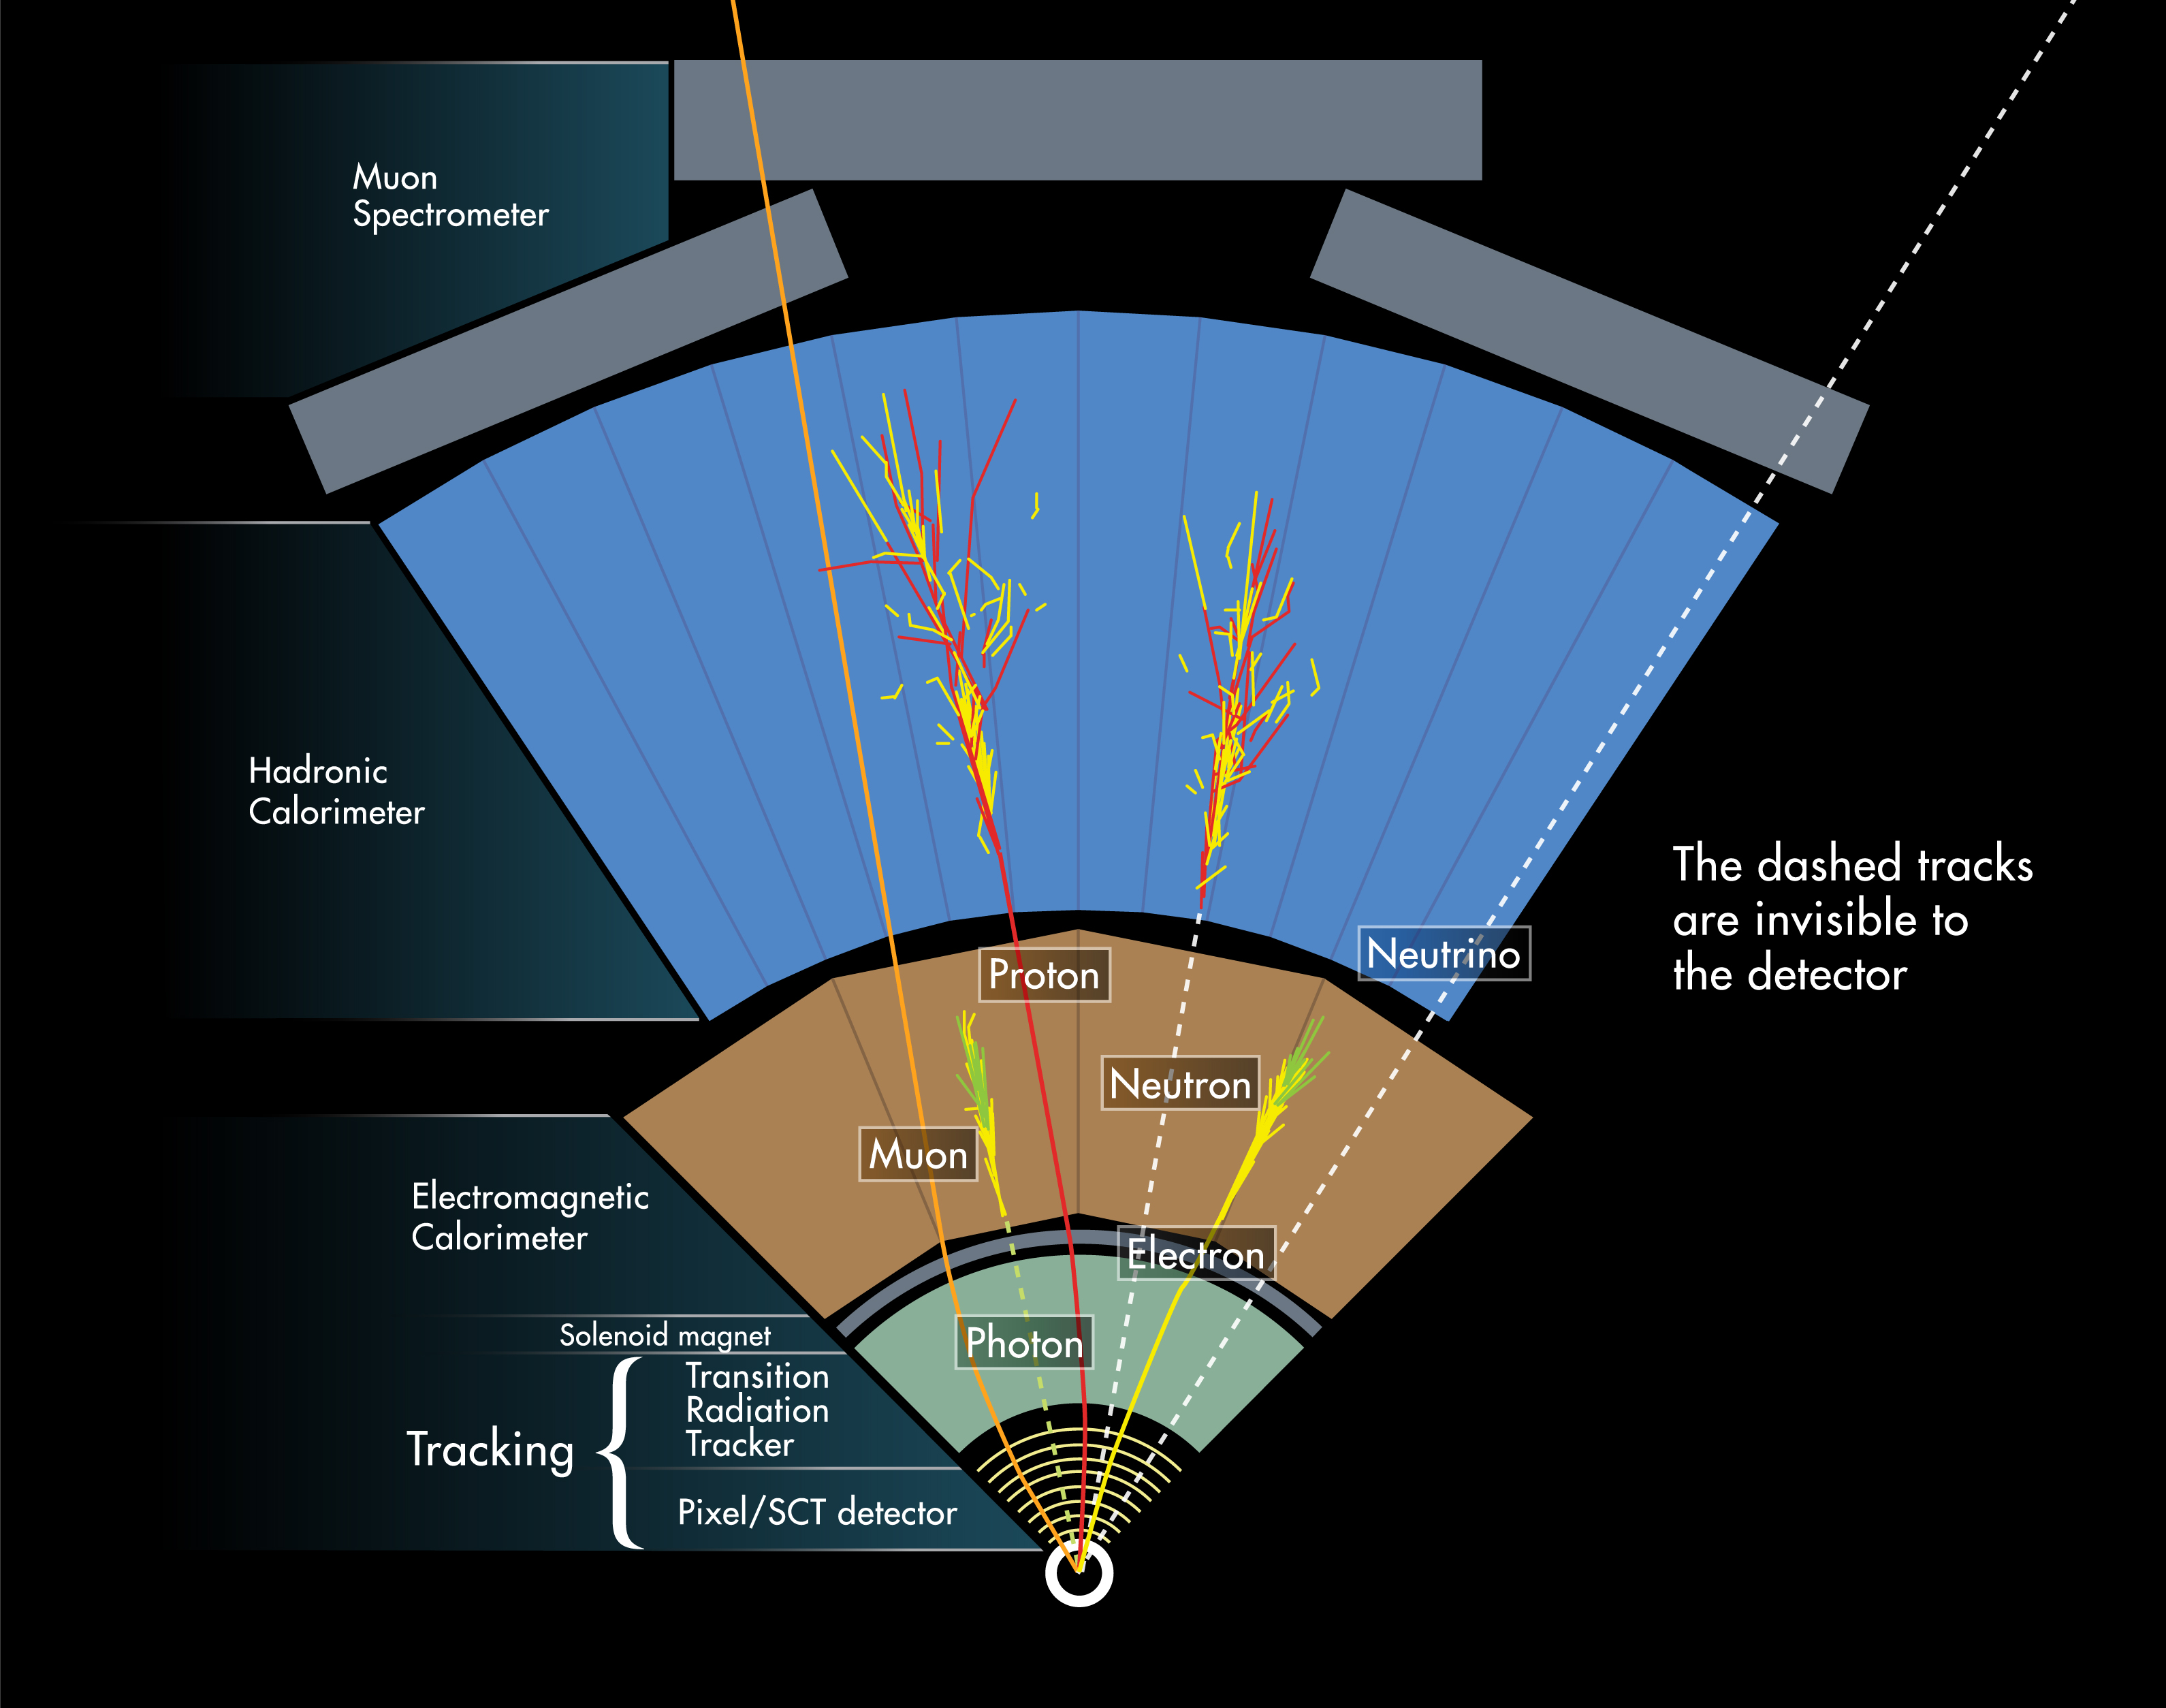
\includegraphics[width=0.85\textwidth, angle=0]{figures/LHC_ATLAS/ATLAS_Signature.jpg}
\caption{ Artistic representation of different detector signatures left by particles in ATLAS.  \label{LHC:fig:ATLASSig}}
%\end{center}
\end{figure}

\indent Details on the reconstruction of physics objects can be found in chapter \ref{chap:reconstruction}.  A brief description of detector signatures will be given here in order to motivate the purpose of each subdetector system. \\

\indent The inner detector provides the position of charged particles as they fly through the detector.  These position measurements are then connected to form a track along the flight path of the charged particle.  A central superconducting solenoid magnet provides a 2 Tesla axial magnetic field that bathes the entire inner detector volume.  The magnetic field bends charged particles in $\phi$ thereby allowing for the measurement of momentum as a function of track curvature.  \\

\indent The calorimeters sample the energy of all charged and neutral particles that interact via the electromagnetic and strong force.   The ATLAS calorimeter is a sampling calorimeter that alternates between absorber and active material layers.   Electromagnetically charged particles such as electrons and photons interact with the dense absorber material mainly through bremsstrahlung, ionization and electron pair production.  An EM particle shower develops until the particles within the shower no longer have the energy necessary to pair produce.  Hadronic particles that interact via the strong force will also form analogous hadronic showers.  The shower particles deposit energy in the active material layers within the calorimeter inducing a signal.  \\


%The particles interact with the dense absorbing material via a number of interactions.  The dominant interaction for electromagnetically charged particles such as the electron is photon emission through bremsstrahlung and ionization.  Neutral high energy photons interact primarily by pair producing electrons.  Any emitted photon and electron will pair produce electrons emit photon until the resulting particles no longer have enough energy to continue the process.  This cascade of particles is called a particle shower.  Hadronic particles that interact via the strong force will also form analogous hadronic showers.  \\

\indent We can measure the longitudinal and lateral shower shape and shower depth by combining signals from different calorimeter layers. Showers from EM objects such as photons and electrons form denser narrow profiles while showers from strongly interacting particles form broad showers that penetrate deep into the hadronic calorimeter. \\

\indent The muon is the only charged SM particle that is expected to be able to fully penetrate the entire calorimeter intact.  Muons in turn leave tracks in the muon spectrometer (MS).  This track can be matched to the inner detector track forming a combined muon track that traverses the entire detector.  Barrel and endcap superconducting toroid magnets provide a magnetic field to the MS volume and allow the momentum measurement.  Field strength varies depending on location but on average an integrated field of 2.5 $T\ddot m$ and 4 $T \cdot m$ are expected for muons traversing through the barrel and endcap respectively.\\

\indent A combination of these different detector signatures is used to identify and reconstruct the different particles produced in a particle collision.  Electrons leave an electromagnetic shower in the calorimeter with an associated track.  Unconverted photons leave an electromagnetic shower without an associated track.  Colored partons fragment into jets and leave a hadronic shower in the calorimeter with a number of associated inner detector (ID) tracks.  Muons are reconstructed from a combined ID and MS track with limited energy deposited in the calorimeter.  Tau leptons either decay leptonically via $\tau \rightarrow \nu \mu \nu$ or $\tau \rightarrow \nu e \nu$ or decay hadronically to pions and leave a narrow hadronic shower in the calorimeter.  Particles that only interact via the weak force, i.e. neutrinos, do not interact with the ATLAS detector.  These weakly interacting particles escape the detector completely and their presence can be inferred through the conservation of transverse momenta as $\met$.\\

\indent The following subsections are dedicated to covering each subdetector in further detail. \\

\subsection{ Inner Detector }
\label{LHC:ID}

\indent The inner detector consists of three independent sub-detectors.  All 3 sub-detectors are immersed in a 2 T axial magnetic field produced by a solenoidal superconducting magnet.  Two silicon semiconductor detectors, the Pixel detector and the Semiconductor Tracker (SCT), form the inner part of the tracking volume and the Transition Radiation Tracker (TRT) covers the outer part.  The three independent sub-detectors together provide a precise and robust pattern recognition system used to reconstruct charged particle tracks and measure charged particle momentum.  The ID also provides precise impact parameter measurements of tracks and primary and secondary vertex reconstruction.   \\

\indent The layout of the inner detector can be seen in Figure \ref{LHC:fig:ATLASID}.  A summary of the geometry and coverage of each ID subdetector is given in Table \ref{tab:IDspec}.  \\

\begin{table}[h!]
  \caption{ Main specifications of each subdetector in the ATLAS inner detector including the intrinsic accuracy of single sensor elements. }
  \label{tab:IDspec}
  \begin{center}
    \begin{tabular}{l c c c} \hline
      Detector & Sensor Element & Avg. num. of hits & $\eta$ coverage \\ 
                     &  Size & per barrel track  & \\ \hline
      IBL         & $50\times240$ $\mu$m$^2$ & 1 & 3.0 \\ 
      Pixel       & $50\times400$ $\mu$m$^2$  & 3 & 2.5\\ 
      SCT        & 80 $\mu$m & 4 & 2.5\\ 
      TRT        &  4 mm & 36 & 2.0 \\ \hline
    \end{tabular}
  \end{center}
\end{table}

\begin{figure}[h!]
%\includegraphics[width=0.45\textwidth, angle=0]{figures/LHC_ATLAS/ID_newTRT_d3.eps}
  \begin{center}
    \begin{subfigure}[a]{0.85\textwidth}   
	\includegraphics[width=\textwidth, angle=0]{figures/LHC_ATLAS/FigID11blast.eps}
         \caption{ }
    \end{subfigure}
    \begin{subfigure}[b]{0.85\textwidth}   
	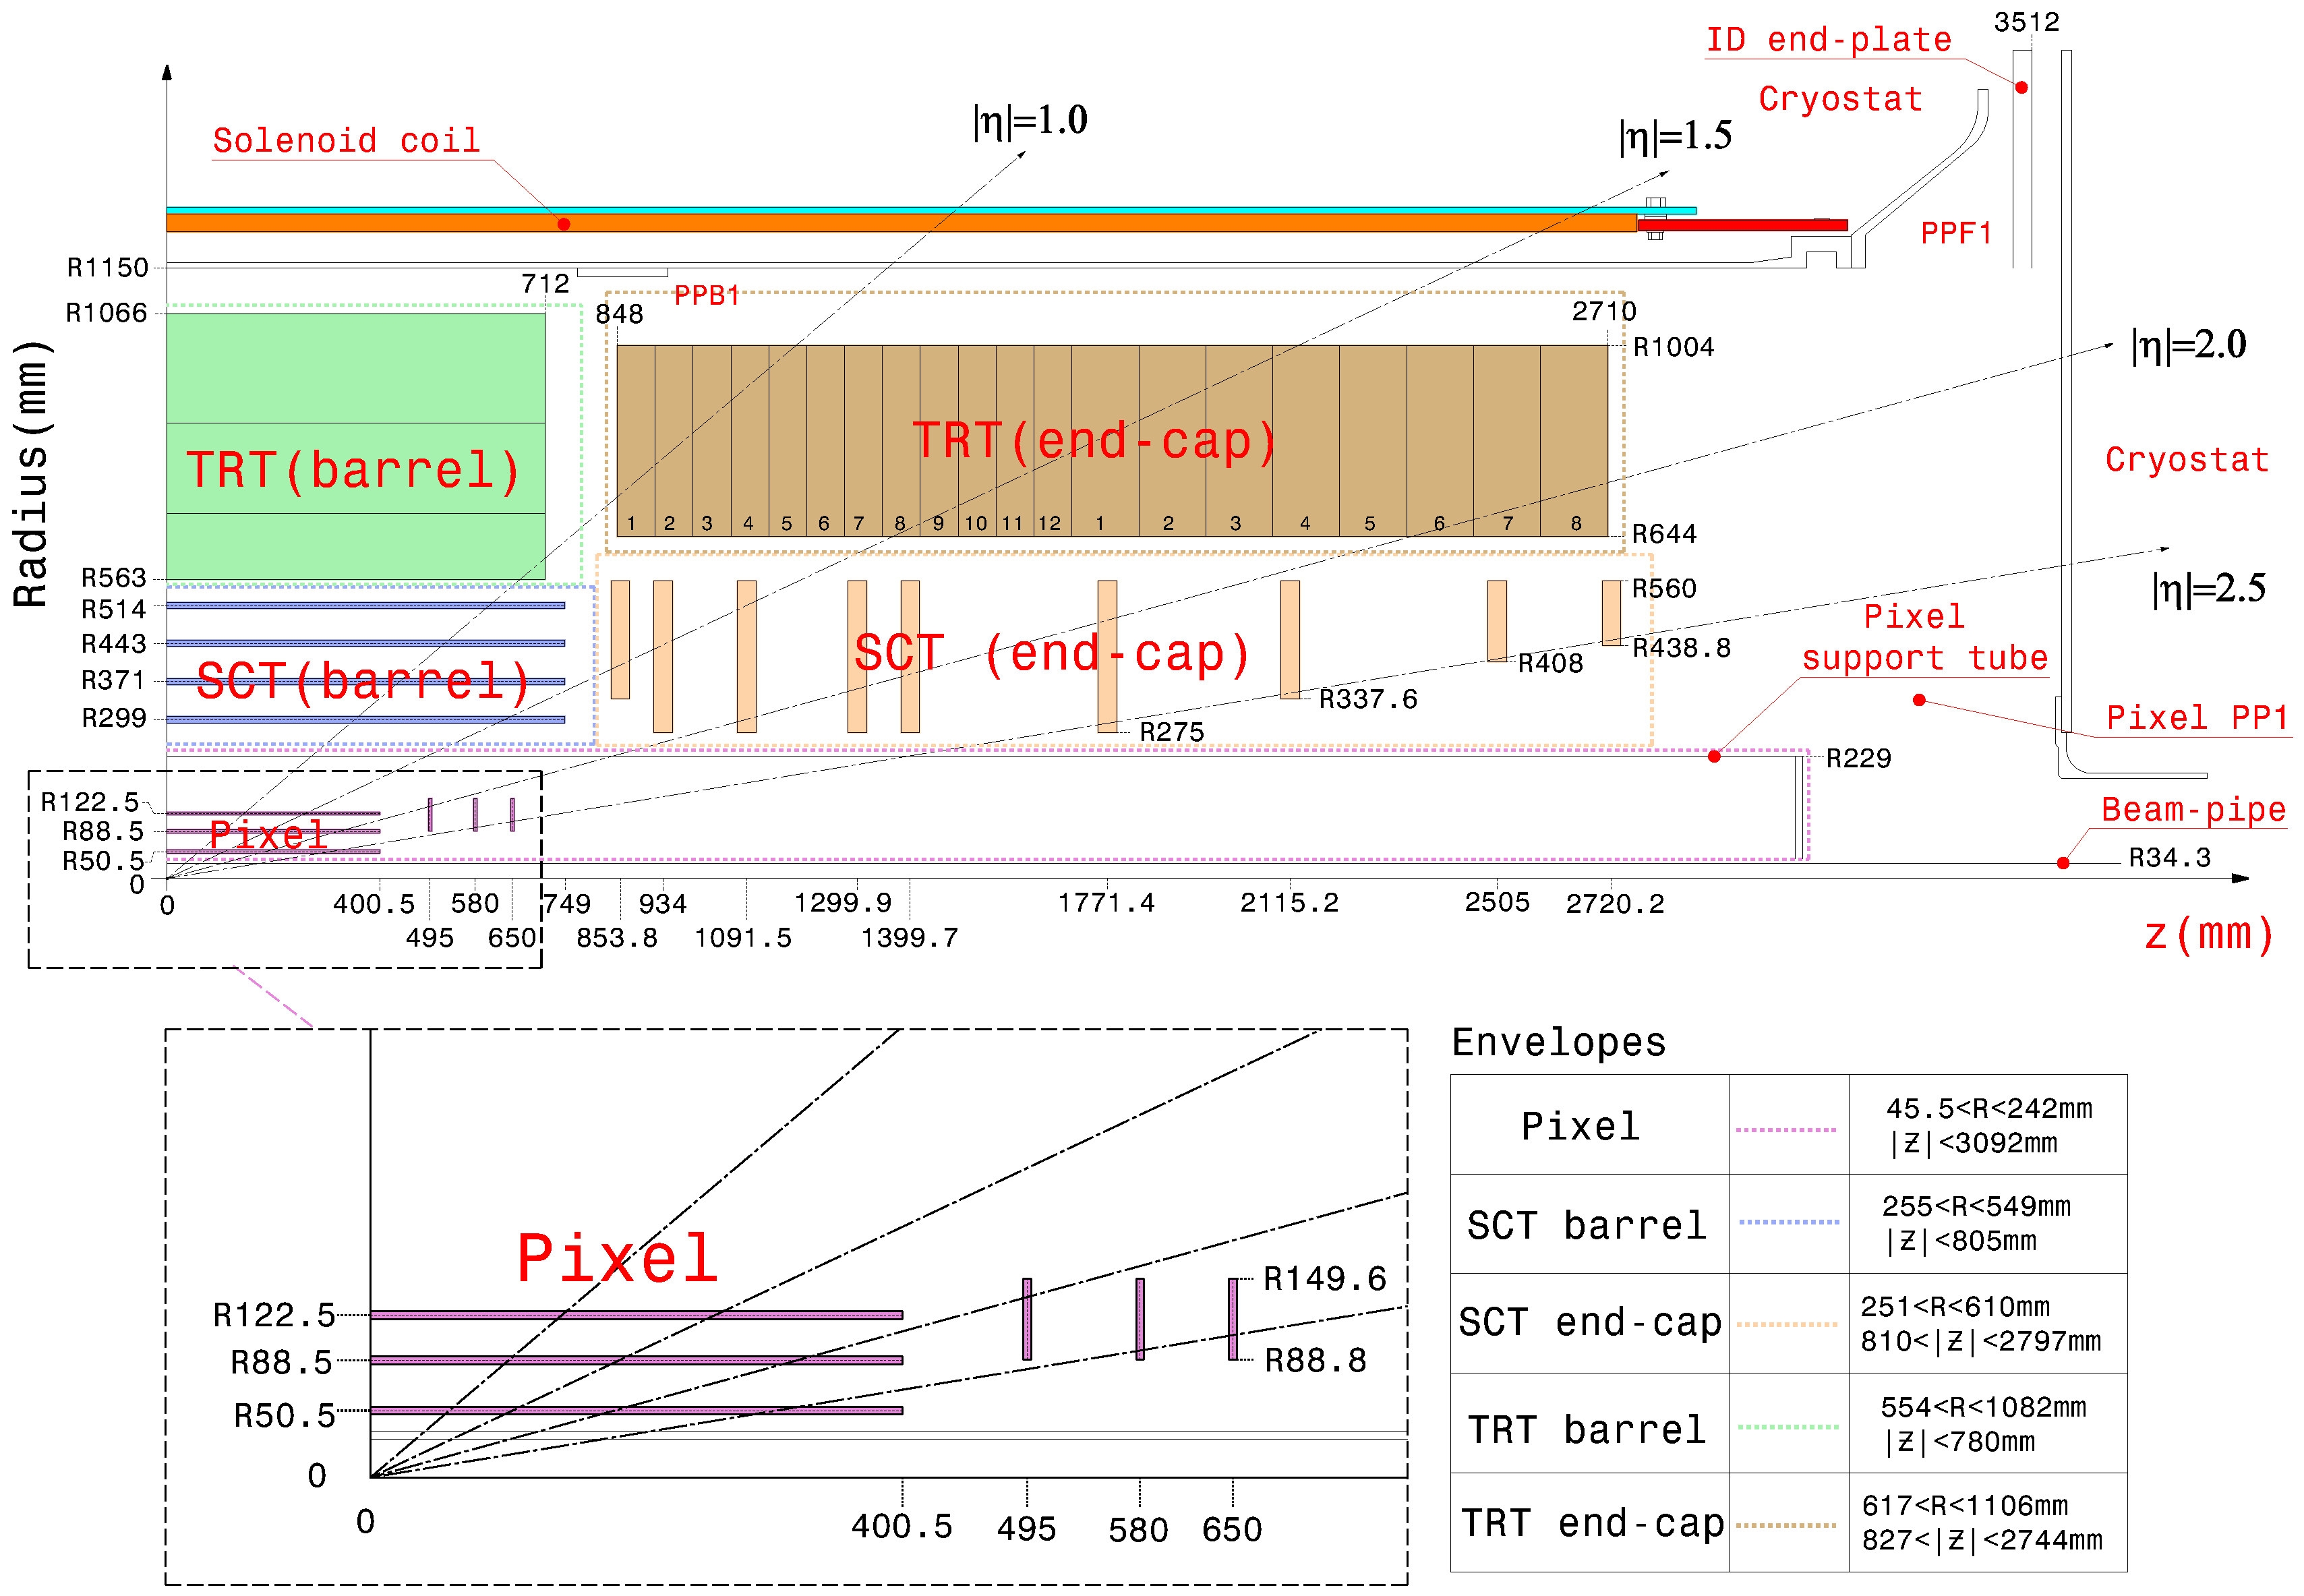
\includegraphics[width=\textwidth, angle=0]{figures/LHC_ATLAS/FigID26-mod-011107.eps}
         \caption{ }
    \end{subfigure}
\caption[~Radial and Cutaway view of the ATLAS inner detector]{ (a) Cutaway view of the ATLAS inner detector. (b) Radial View of the ATLAS inner detector. \cite{ATLAS_JINST} \label{LHC:fig:ATLASID}}
\end{center}
\end{figure}

\indent More detail on each ID sub-detector technology is given below. \\

\subsubsection*{ Pixel Detector and the Insertable B-Layer}

\indent The Pixel detector consists of three layers of high resolution pixel silicon sensors in the cylindrical barrel and three wheels of pixel sensors in the endcap.  The innermost layer of pixel sensors, called the Insertable B-Layer (IBL), was added in the first long shutdown between 2012 and 2015 along with a new beryllium beam pipe.  The new beam pipe decreases the amount of multiple scattering before the inner tracker. \\

\indent The original 3 layer Pixel detector comprises 80.4 million readout channels spread over 1744 Pixel modules.  Each module houses a sensor tile with an area of $63.4 \times 25.4$ mm$^2$.  The sensors are composed of 250 $\mu$m thick n-type silicon wafer pixels with a size of $50\times400 \mu$m$^2$. The modules are read out by 16 front-end electronic chips, each with 2880 read out channels. \\

\indent The pixels have an intrinsic accuracy of 10 $\mu$m in the bending $\phi$ direction and 115 $\mu$m accuracy in the non-bending $z$ direction in the barrel and $\phi$ direction in the endcap.\\ 

\indent Installed in 2014, the Insertable B-Layer (IBL) contributes another 12 million channels to the Pixel system in Run 2.\cite{IBLOverview,IBL_TDR}  Located directly on top of the beam pipe at 3.3 cm from the beam axis, the IBL is the new most inner layer of the Pixel detector ( the previous innermost B-Layer was at 5 cm ). A schematic representation of IBL stave relative to the beam pipe can be seen in Figure \ref{LHC:fig:IBL}. \\

\begin{figure}[h!]
%\begin{center}
\centering
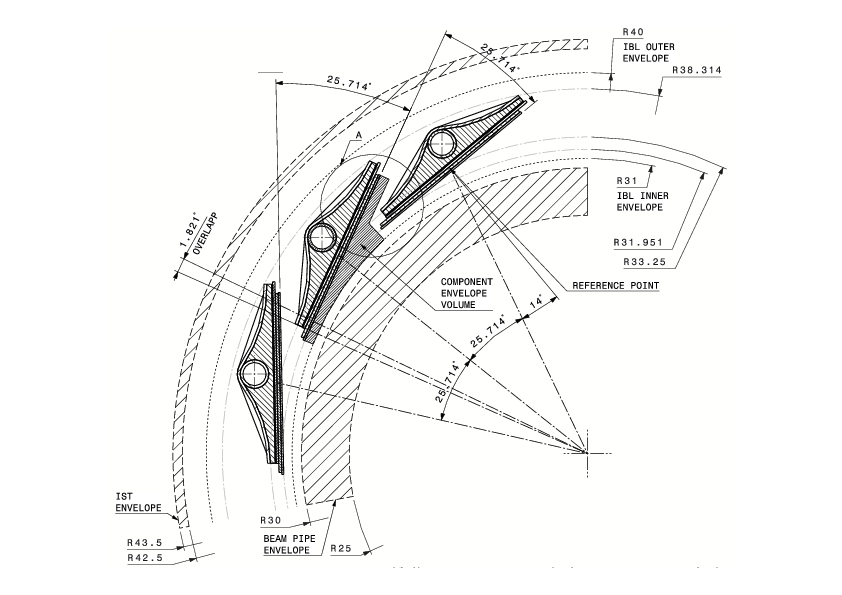
\includegraphics[width=0.85\textwidth, angle=0]{figures/LHC_ATLAS/fig_ibl_layout_rev.png}
\caption[~Schematic of the ATLAS Insertable B-Layer (IBL)]{ Schematic of the ATLAS Insertable B-Layer (IBL).\cite{IBLOverview} \label{LHC:fig:IBL}}
%\end{center}
\end{figure}

\indent The IBL is composed of 14 staves tilted at $14^{\circ}$ in $\phi$.  Each stave is equipped with 32 FE-I4 front-end chips bonded to silicon sensors. Each FE-I4 chip contains 26880 pixel cells with $50 \times 240$ $\mu$m$^2$ pitch.\\

\indent The IBL improves both the tracking lever arm and track spatial resolution.  The combined improvements translate to a factor of $\sim2$ improvement in the impact parameter resolution and a factor of $\sim4$ improvement in the b-tagging light jet rejection power. \\

\subsubsection*{ Semiconductor Tracker}

\indent The SCT is composed of 4 coaxial layers of concentric cylinders in the barrel and 9 disks in each endcap and contributes at least 4 additional layers of high precision position measurements to tracks.  The entire SCT consists of approximately 6.3 million readout channels spread over 4088 modules.  A barrel module is equipped with $64.0 \times 63.6$ mm$^2$ sensors orientated in the transverse plane.  Barrel sensors are made of 285 $\mu$m thick silicon wafers and contain 768 strips, achieving a barrel strip-pitch of 80 $\mu$m.  The endcap modules contain sensors that are trapezoidal in shape with strip pitch that vary from 54 $\mu$m to 90 $\mu$m.  \\

\indent The sensors are mounted in a back-to-back fashion at angle of $40$ mrad relative to one another.  This allows the measurement of non-bending direction along with improved spatial resolution in the bending $\phi$ direction. The intrinsic accuracy per SCT module, dictated by the strip pitch, is 17 $\mu$m in the bending $\phi$ direction and 580 $\mu$m in the non-bending direction.\\

\subsubsection*{Transition Radiation Tracker}

\indent The TRT is the outermost component of the ID and contributes approximately 351000 readout channels.  Each channel corresponds to a 4 mm diameter polyimide straw drift tube with a $31 \mu$m gold plated tungsten anode wire, providing an intrinsic accuracy of 130 $\mu$m.  The total channel number is low compared to the silicon detectors but the TRT is able to compensate for this by providing a long lever arm and high hit multiplicity.  \\

\indent In the barrel region, TRT straws are 144 cm long and arranged parallel to the beam axis in 73 layers. In the end-cap region, straws are 37 cm long and arranged in wheels with 160 radial layers.  A typical barrel track will traverse 36 straws because the tubes are arranged in a matrix with layers offset from one another.\\

\indent The dielectric material used to interweave the straws induces transition radiation in traversing charged particles.  The Xenon-based gas mixture in the straws absorbs the low energy transition radiation photons. The transition radiation thereby induces a much larger signal amplitude than a minimum-ionizing charged particle.  The large signal can then be used to distinguish electrons from charged pions.  \\

\indent In 2015 and 2016, approximately $1/3$ to $2/3$ of the TRT barrel and $1/7$ of the TRT endcap were filled with an Argon gas mixture instead of Xenon due to leakages.  This decreased electron identification efficiency by a few percent during 2015 and 2016.  This decrease in electron identification efficiency is taken into account by a scale factor in the simulation.  \\

\subsection{The Calorimeter}
\label{LHC:Calorimeter}

\indent The ATLAS calorimeter provides near full solid angle coverage of the interaction point up to an $|\eta| < 4.9$.  The calorimeter system is composed of two parts; the electromagnetic calorimeter (ECAL) and hadronic calorimeter (HCAL).  Both ECAL and HCAL are sampling calorimeters with different absorber material depending on the detector region.  The ECAL uses liquid argon (LAr) as the active material and HCAL uses both scintillating tiles and liquid argon (LAr) as active materials.  \\

\indent The cutaway view of the ATLAS calorimeter can be seen in Figure \ref{LHC:fig:ATLASCalo}. \\% and a summary of the calorimeter geometry is given in table \ref{} \\

\begin{figure}[h!]
%\begin{center}
\centering
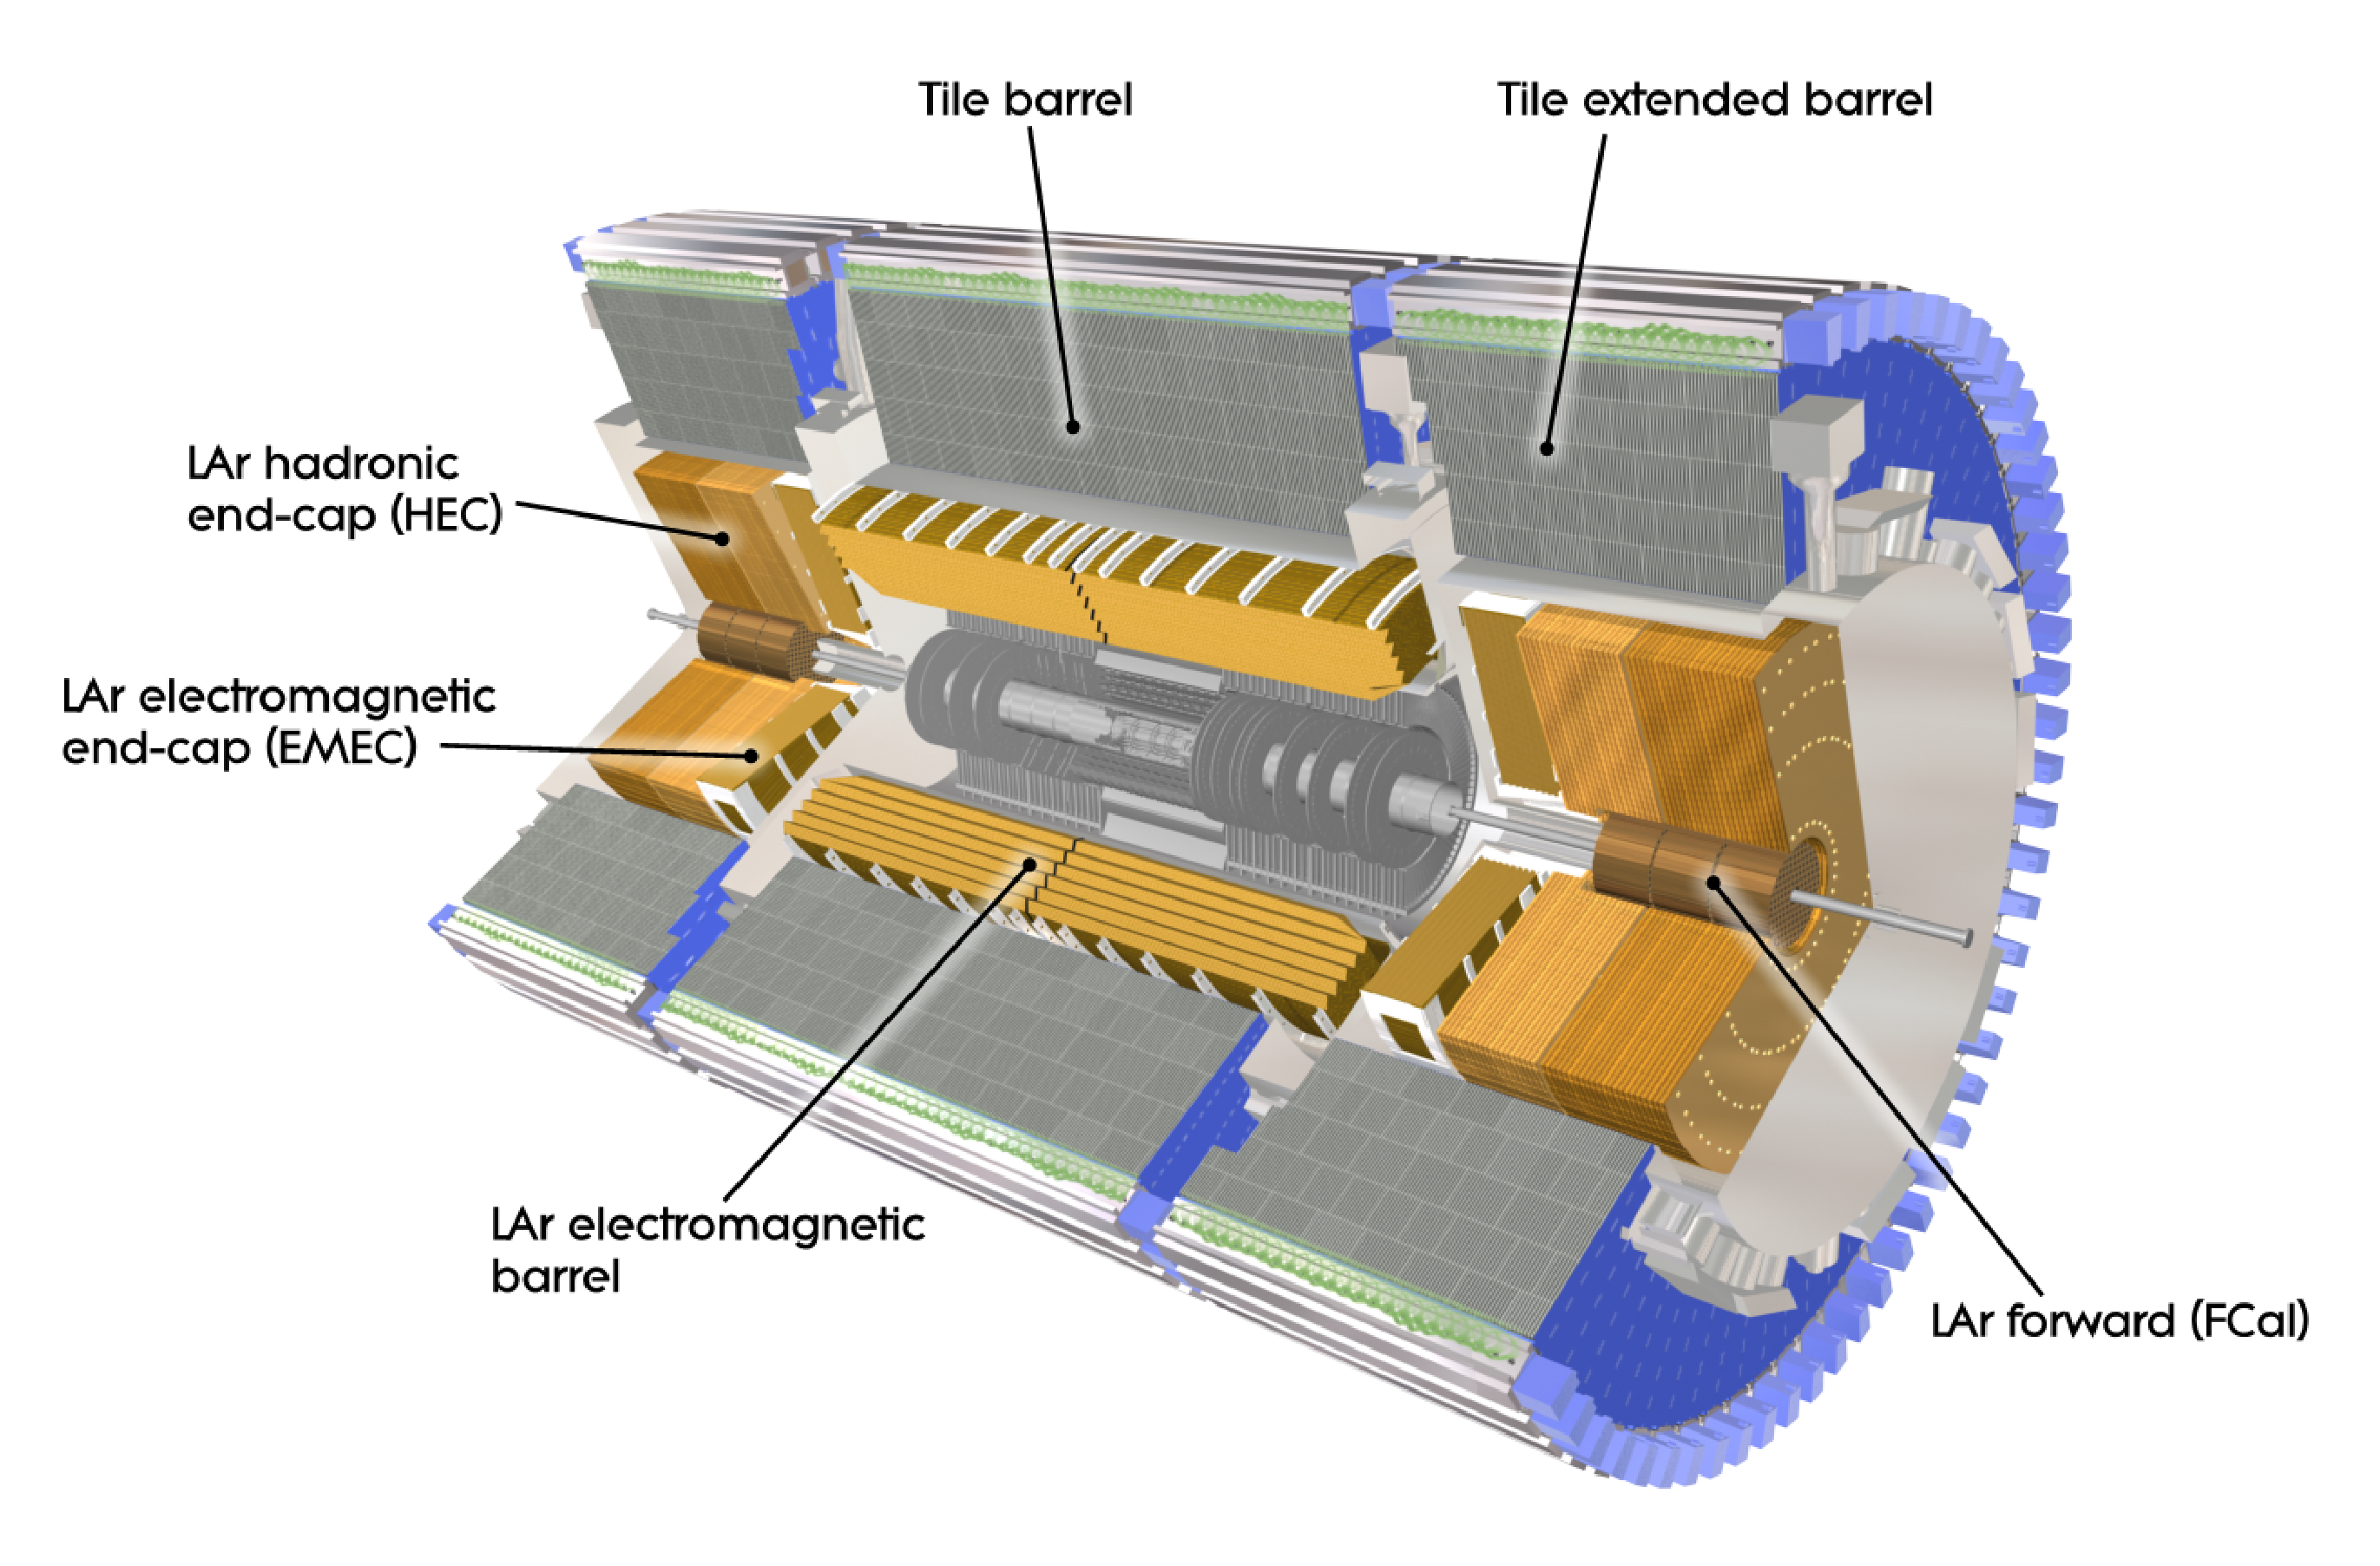
\includegraphics[width=0.75\textwidth, angle=0]{figures/LHC_ATLAS/Calorimeter_d3.eps}
\caption[~Layout of the ATLAS calorimeter]{ Layout of the ATLAS calorimeter.\cite{ATLAS_JINST} \label{LHC:fig:ATLASCalo}}
%\end{center}
\end{figure}

\indent The design EM resolution is $\sigma_E/E = 10\%/\sqrt{E} \oplus 0.2\%$. The design hadronic energy resolution varies from $\sigma_E/E = (56.4\pm0.4)/\sqrt{E}\oplus(5.4\pm0.1)$\% in the barrel region to $\sigma_E/E = (94.2\pm1.6)/\sqrt{E}\oplus(7.5\pm0.4)$\% in the forward regions. \\

\subsubsection*{Electromagnetic Calorimeter}

\indent The ATLAS ECAL is sampling calorimeter with lead absorber plates and LAr active material arranged in an accordion geometry.  The ECAL provides coverage up to an $|\eta| < 3.2 $ and the accordion design gives full crack-less coverage in $\phi$. \\% and integrates more charge along the longitudinal direction of the shower.  \\

\indent The ECAL is split into a barrel and two endcap components with a transition region of $1.37 < |\eta| < 1.52$ in between.  The barrel component is divided into two 3.2 m long half-barrel sections with an inner and outer radius of 2.8 m and 4 m respectively.  The endcap is divided into two coaxial wheels each 63 cm thick with an outer wheel covering the $1.375 < |\eta| < 2.5$ region and an inner wheel covering the $2.5 < |\eta| < 3.2$ region. \\

\indent The barrel ECAL is segmented longitudinally into 3 layers with an additional presampler layer in front of certain regions.  The presampler is composed of a thin liquid-argon layer 11mm in depth and is designed to determine the energy loss from material upstream of the calorimeter.  The first layer after the presampler has a depth of 4.3 radiation length ($\Chi_0$) and a fine granularity with $\Delta\eta \times \Delta\phi = 0.003 \times 0.1$.  The high granularity allows for precision measurement of EM showers and can distinguish between the shower shape of electron/photons from those of $\pi^0\rightarrow \gamma\gamma$ decays.  The middle layer absorbs most of the energy in the EM shower and is made up of cells with $\Delta\eta \times \Delta\phi = 0.025 \times 0.025$ and a depth of $16 \Chi_0$.  The back layer is designed to collect the tails of the EM showers and to distinguish between EM and hadronic showers. The back layer has cell sizes of $\Delta\eta \times \Delta\phi = 0.05 \times 0.025$ and a depth of $2 \Chi_0$.  \\

\indent The endcap ECAL is also divided into three longitudinal layers that perform the functions as the layers in the barrel.  The front layer has a depth of 4.4 $\Chi_0$ and varies in cell size from $\Delta\eta \times \Delta\phi = 0.003 \times 0.1$ to $\Delta\eta \times \Delta\phi = 0.006 \times 0.1$. The middle layer has cells with the same size as the barrel at $\Delta\eta \times \Delta\phi = 0.025 \times 0.025$ and a similar depth. The back layer also has a $\Delta\eta \times \Delta\phi$ of $0.05 \times 0.25$.  A presampler also exists for the endcap with each presampler module consisting of two 2mm thick LAr layers. \\

\indent The ATLAS ECAL segmentation can be seen in Figure \ref{LHC:fig:EMCalo}. \\

\begin{figure}[h!]
\begin{center}
    \begin{subfigure}[b]{0.40\textwidth}   
        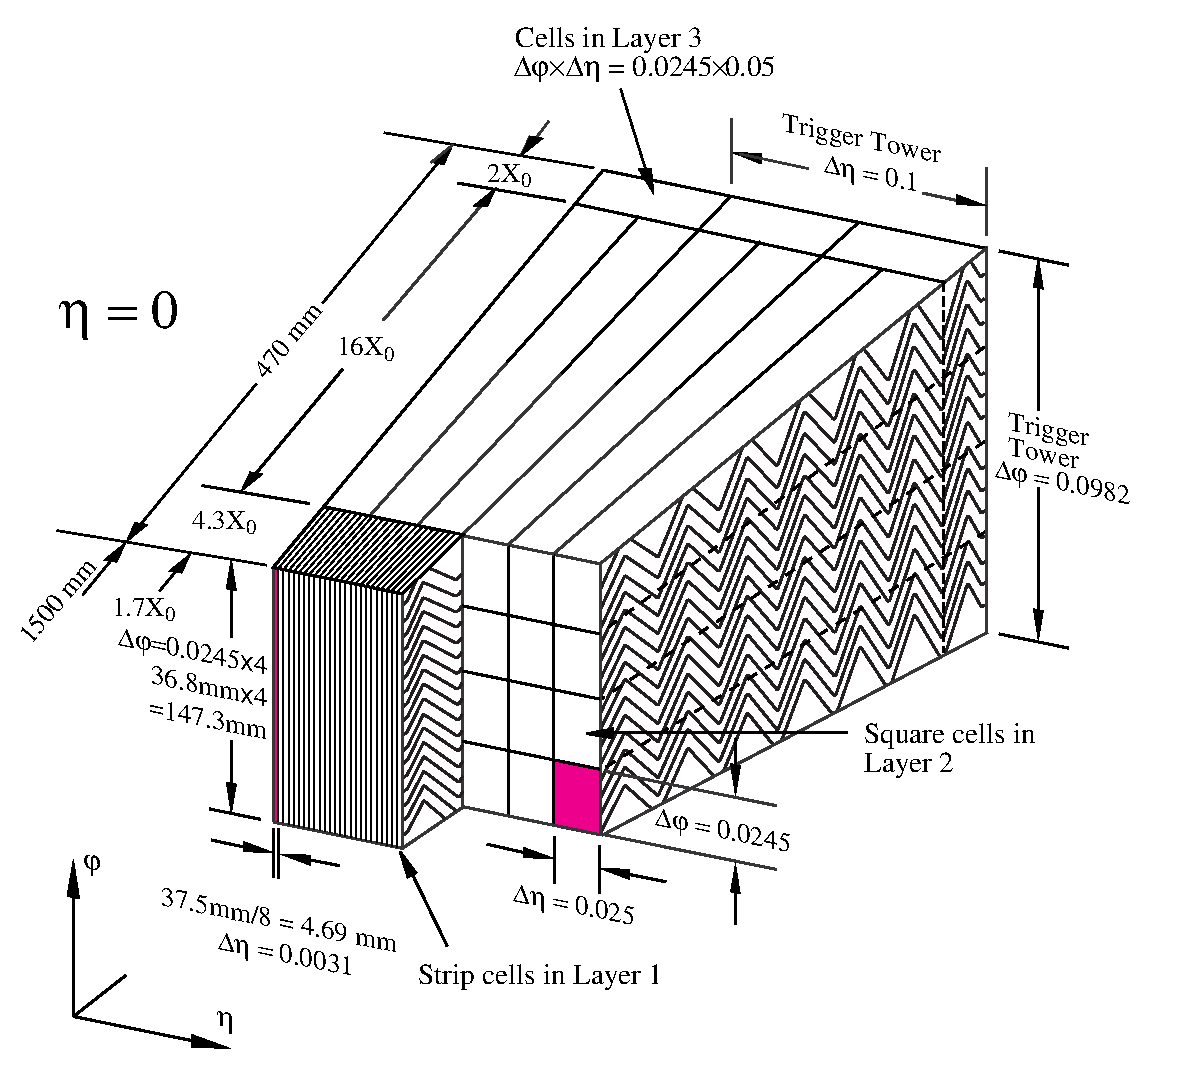
\includegraphics[width=\textwidth, angle=0]{figures/LHC_ATLAS/LARG3-TDR-barrelM.eps}
        \caption{}
    \end{subfigure}
    \begin{subfigure}[b]{0.50\textwidth}
	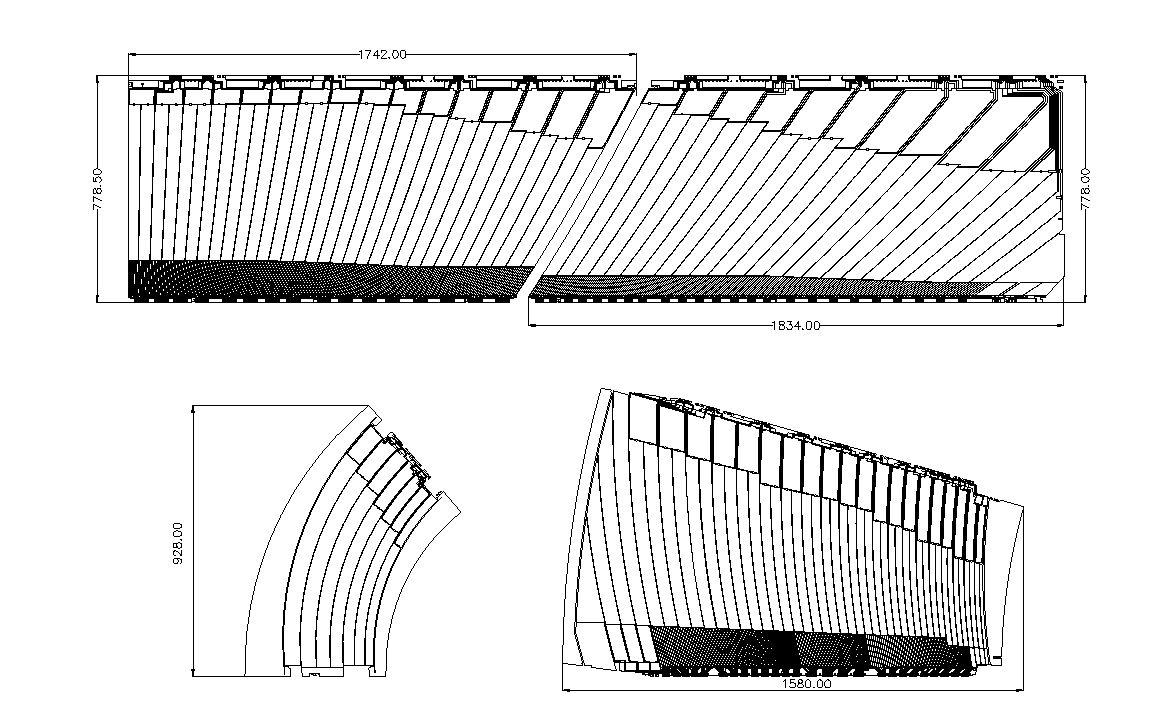
\includegraphics[width=\textwidth, angle=0]{figures/LHC_ATLAS/LARG3-abcdM.eps}
	\caption{}
    \end{subfigure}
\caption[~Schematic depiction of the ATLAS electromagnetic calorimeter module and cells]{ Schematic depiction of the ATLAS electromagnetic calorimeter (a) The three layers of the EM calorimeter module with the accordion geometry shown. (b) Orientation of EM calorimeter cells in the barrel and endcap relative to the IP.  Cells are orientated to point back to the IP.\cite{ATLAS_JINST} \label{LHC:fig:EMCalo}}
\end{center}
\end{figure}

\indent The total thickness of the ECAL is at least $22 \Chi_0$ in the barrel and $24 \Chi_0$ in the endcap for electrons and photons and approximately 1.5 nuclear interaction length for hadronic objects. \\

\subsubsection*{Hadronic Calorimeter}

\indent The ATLAS HCAL is directly outside the ECAL and is responsible for containing and measuring the energy of hadronic showers.  The HCAL consists of 3 separate detectors covering different $\eta$ regions. The tile calorimeter covers the central region with $|\eta| < 1.7$.  The LAr endcap calorimeter (HEC) covers the endcap region with $1.5<|\eta| < 3.2$ and the LAr forward calorimeter (FCal) covers the forward region to upwards of $|\eta| < 4.9$.  \\

\indent The tile calorimeter is a sampling calorimeter using steel absorbers and scintillating tiles as active material. Two separate photomultiplier tubes read out the two sides of the scintillating tiles.  \\

\indent The barrel tile calorimeter covers an $\eta$ range of $|\eta| < 1.0$ and two extended barrel tile calorimeters cover the $0.8 < |\eta| < 1.7$ region.  Both barrel and extend barrel calorimeters are divided into 64 modules orientated along the $\phi$ direction.  Each module covers a $\phi$ region of $\Delta\phi = 0.1$.  The module is segmented in the radial direction into 3 longitudinal layers.  The 3 layers have an approximate thickness of 1.5, 4.1 and 1.8 nuclear interaction lengths ($\lambda$) in the barrel and 1.5, 2.6, and 3.3 $\lambda$ in the extended barrel.  

\indent A Schematic view of a tile calorimeter module can be seen in Figure \ref{LHC:fig:TileCalo}

\begin{figure}[h!]
%\begin{center}
\centering
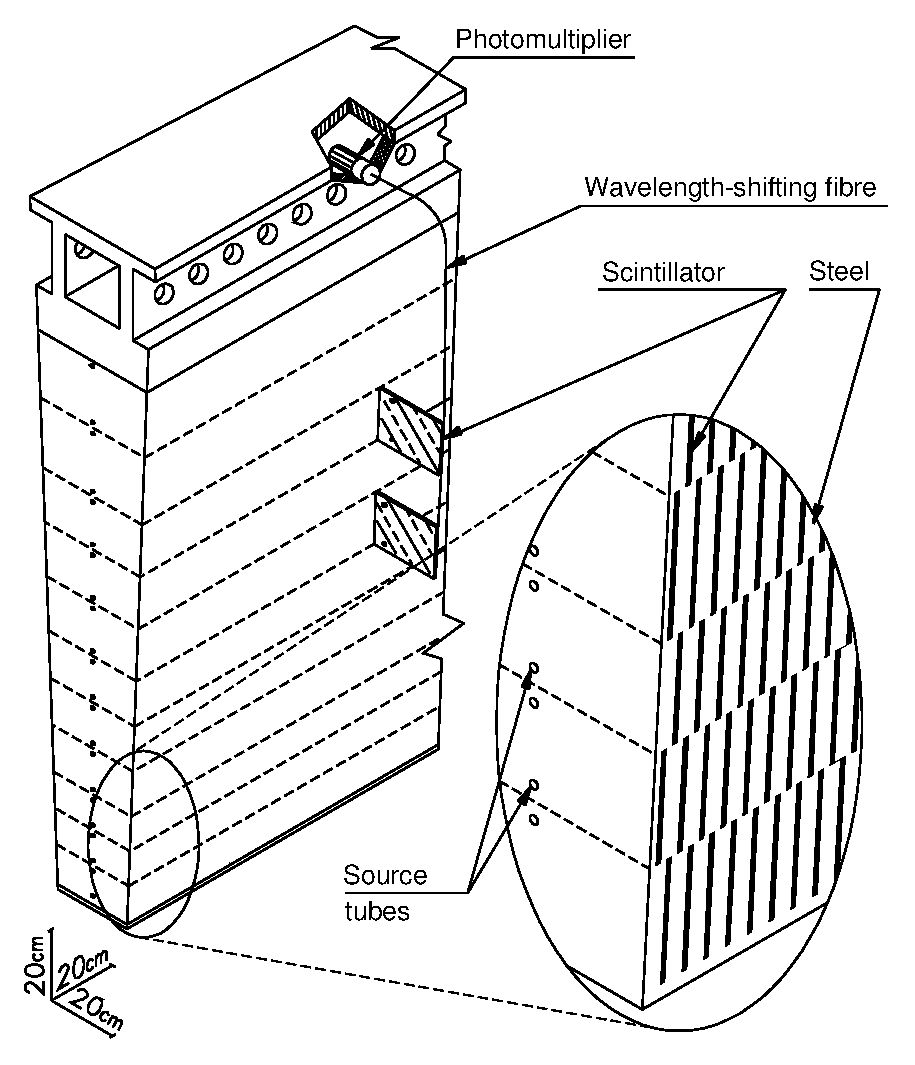
\includegraphics[width=0.45\textwidth, angle=0]{figures/LHC_ATLAS/TileCal_Module3.eps}
\caption[~The tile calorimeter module with steel absorber, tile scintillators and photomultiplier readout]{ The tile calorimeter module with steel absorber, tile scintillators and photomultiplier readout.\cite{ATLAS_JINST} \label{LHC:fig:TileCalo}}
%\end{center}
\end{figure}


\indent The HEC uses LAr as the active material and copper as the absorber with copper plates interwoven between the LAr gaps.  The HEC is located directly behind the ECAL endcap and two calorimeters share a single cryostat.  The HEC  covers an $\eta$ range of $1.5<|\eta| < 3.2$ and overlaps slightly with the tile calorimeter and FCAL in order to minimize any drop in material density.  \\

\indent Geometrically the HEC consists of two independent wheels per endcap with each wheel subdivided into 32 wedge shaped $\phi$ modules.  Each HEC module is composed of cells with a size of $\Delta\eta \times \Delta\phi = 0.1 \times 0.1$ for the $|\eta|<2.5$ region and $\Delta\eta \times \Delta\phi = 0.2 \times 0.2$ in higher eta regions.  The HEC module is also segmented longitudinally into 2 layers making a total of 4 longitudinal layers in the 2 wheels. The combined depth of all 4 layers is approximately 10 interaction lengths. \\

\indent The FCal is an LAr sampling calorimeter that extends the $\eta$ coverage of the HCAL up to $|\eta| < 4.9$.  A compact design with very small LAr gaps is chosen for this high flux region.  The FCal is segmented in the longitudinal direction with 3 distinct modules. The absorber material is copper for the first module and tungsten in the last two.  The copper absorber is optimized for EM measurements while the tungsten is predominantly designed for hadronic interactions.  The 3 modules combined achieve a depth of 10 nuclear interaction length. \\

\subsection{The Muon Spectrometer}
\label{LHC:MuonSpec}

\indent The muon spectrometer (MS) consists of three layers of precision tracking chambers to track the path of muons in the bending $\eta$ direction.  The precision tracking chambers mainly consists of Monitored Drift Tube (MDT) detectors but also includes Cathode Strip Chambers (CSC) in the forward region.  Complementing the precision trackers are fast trigger chambers, the Resistive Plate Chambers (RPC) in the barrel and the Thin Gap Chambers (TGC) in the endcap. \\


\indent The MS is designed to be able to detect muon candidates with a wide range of momenta from $3 \gev$ to $3 \tev$ with standalone muon momentum resolution of $\sigma_{\pt}/\pt = 10\%$ at a $\pt$ of 1 TeV.  The configuration of the MS is shown in Figure \ref{LHC:fig:ATLASMuonSpec}.  The open design of the MS minimizes multiple scattering after the calorimeter and gives a large lever arm for high momentum resolution. ~\\

\begin{figure}[h!]
%\begin{center}
\centering
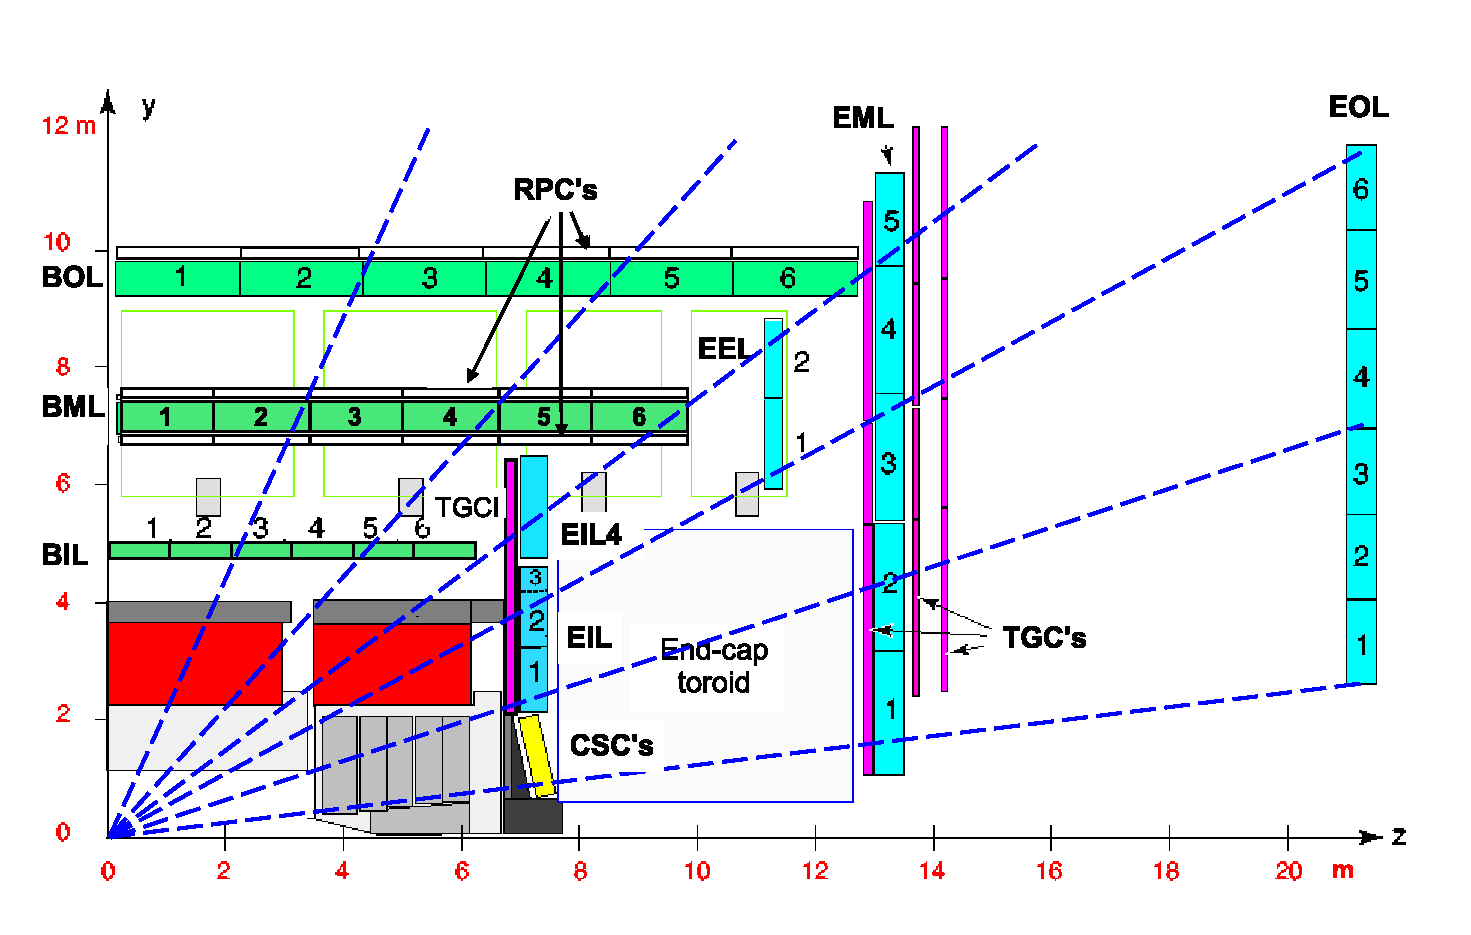
\includegraphics[width=0.75\textwidth, angle=0]{figures/LHC_ATLAS/Muon_rz_large_sect_6.eps}
\caption[~Cutaway view of the ATLAS Muon Spectrometer]{ Cutaway view of the ATLAS Muon Spectrometer.\cite{ATLAS_JINST} \label{LHC:fig:ATLASMuonSpec}}
%\end{center}
\end{figure}

\indent Eight air core superconducting toroid magnets in the barrel and eight additional magnets in each endcap provide a 1.0 $T \cdot m$ to 7.5 $T \cdot m$ of bending power in the MS volume. The configuration of the magnets is shown in Figure \ref{LHC:fig:ATLASMag} ~\\

\begin{figure}[h!]
%\begin{center}
\centering
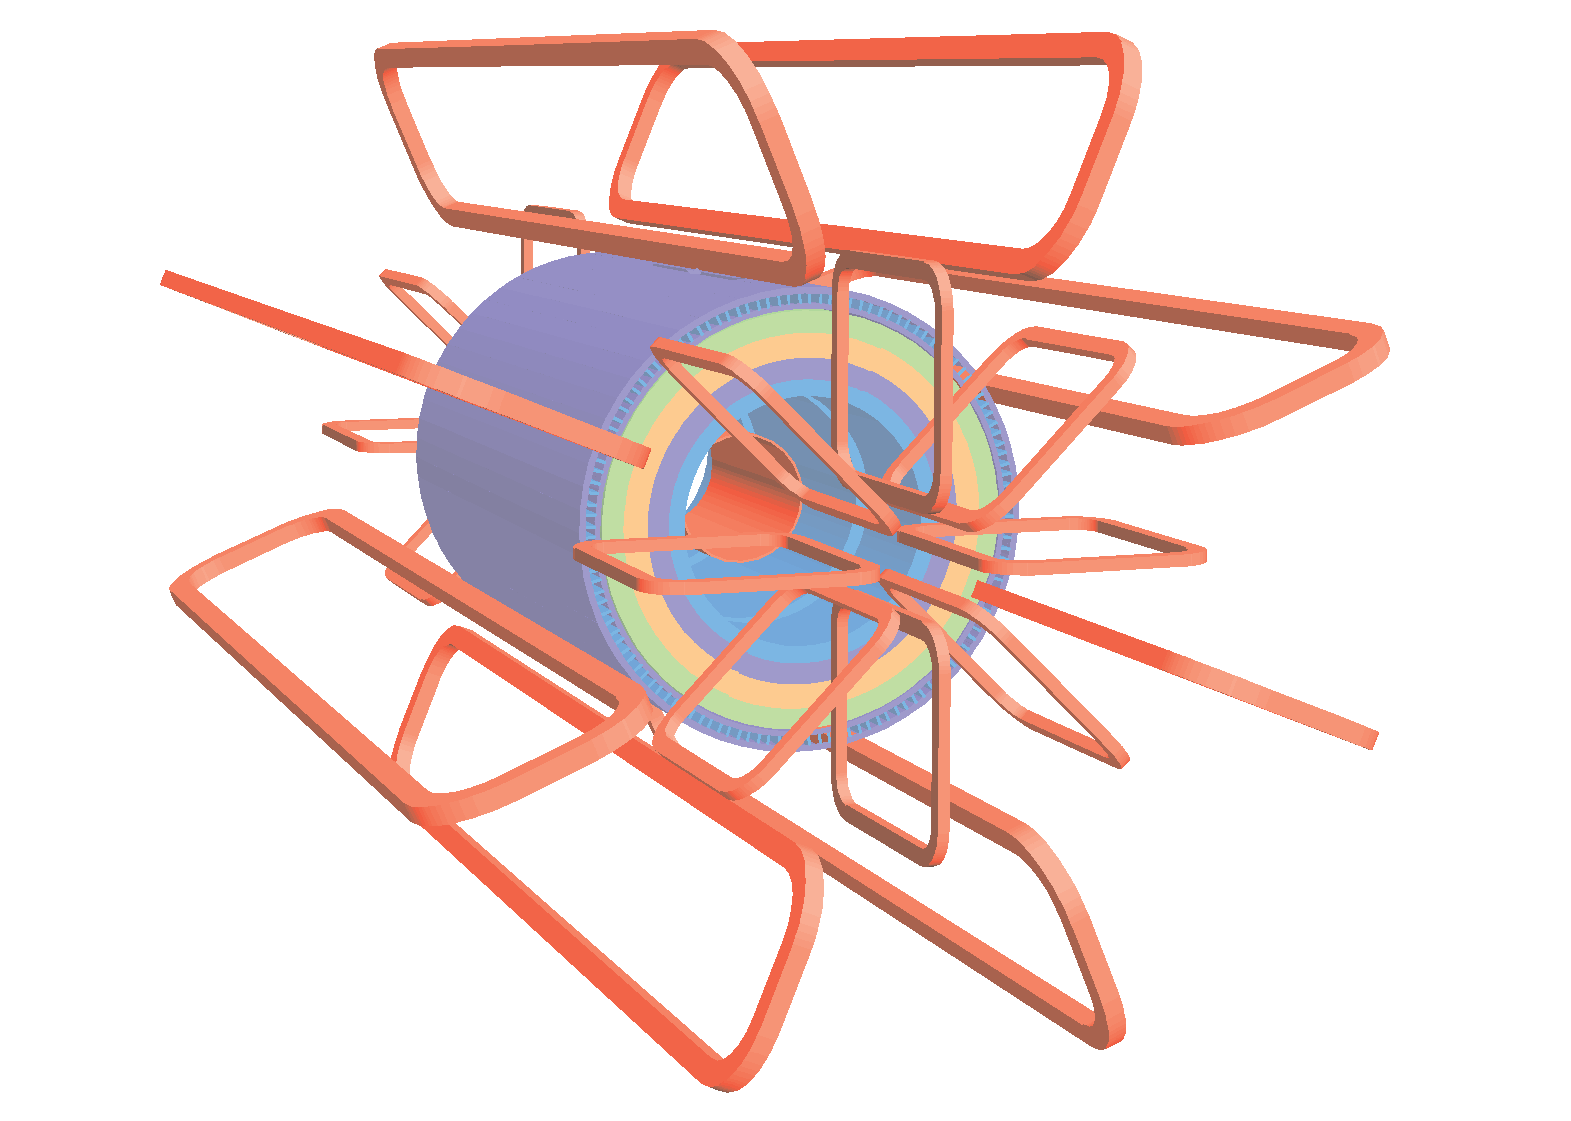
\includegraphics[width=0.60\textwidth, angle=270]{figures/LHC_ATLAS/ATLcoilGeom.eps}
\caption[~Geometry of the ATLAS barrel and endcap toroid magnets]{ Geometry of the ATLAS barrel and endcap toroid magnets. The cylinder represents the calorimeter.\cite{ATLAS_JINST} \label{LHC:fig:ATLASMag}}
%\end{center}
\end{figure}

\indent The barrel magnets cover an |$\eta$| range up to 1.4 and the endcap magnets cover an |$\eta$| range from 1.6 to 2.7. The area between $1.4 < |\eta| < 1.6$, called the transition region, has a mixed magnetic field from both the barrel and endcap. The endcap magnets are offset from the barrel magnets by 22.5 degrees in $\phi$ to allow a smoother magnetic field in the transition region. \\

\subsubsection*{Muon Precision Tracking}

\indent The ATLAS MS system consists of 3 stations of muon precision tracking chambers at approximately 5 m, 7.5 m and 10 m radii in the barrel and 7.4 m,14 m and 21.5 m in $z$ in the endcap.  This provides precision tracking coverage up to an $|\eta| < 2.7$.  Most precision tracking chambers use Monitored Drift Tube (MDT) technology with 3 to 8 layers of MDT tubes each.  The only exception to this is the very high rate forward region with $2.0 < |\eta| < 2.7$ which uses CSC technology. \\

\indent  MDT tubes are 3cm diameter aluminum tubes filled with Ar/CO$_2$ gas mixture with a tungsten-rhenium anode wire.  Each tube has an intrinsic resolution of 80 $\mu$m corresponding to a resolution of $35$ $\mu$m per chamber and offers position measurements in the bending $\eta$ direction.  \\

\indent The CSCs are multiwire proportional chambers with one layer of anode wires in the bending plane and two layers of cathode strips. The position measurement is obtained by interpolating the signal on neighboring cathode strips. The strips are perpendicular to one another with 5.31mm (5.56mm) pitch in the bending plane and 12.5 mm (21.0 mm) in the non-bending plane for small (large) chambers.   This results in a $60 \mu$m resolution per plane in the bending plane and about 5 mm resolution in the non-bending plane. \\ %The CSC wire signals are not read out.    The primary limiting factor for the CSC spatial resolution is electronic noise of the pre-amplifiers and not strip pitch. 

\indent The structure of MDT tubes and CSC chambers can be seen in Figures \ref{LHC:fig:MDT} and \ref{LHC:fig:MDT} . \\

\begin{figure}[h!]
%\begin{center}
\centering
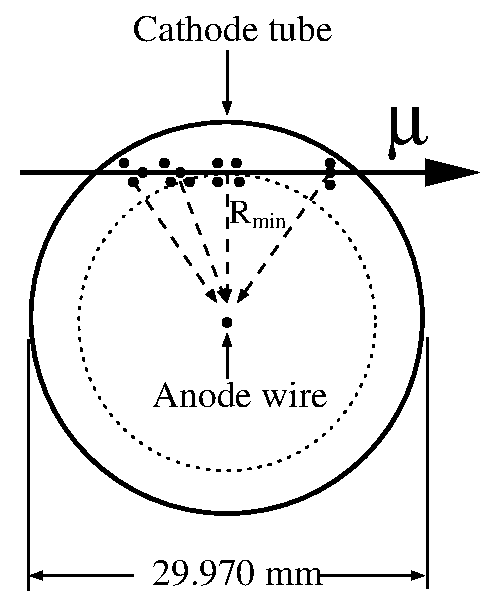
\includegraphics[width=0.30\textwidth, angle=0]{figures/LHC_ATLAS/MDT_tube_cross_section.eps}
\caption[~Schematic Representation of MDT tubes]{ Schematic Representation of MDT tubes.\cite{ATLAS_JINST} \label{LHC:fig:MDT}}
%\end{center}
\end{figure}

\begin{figure}[h!]
%\begin{center}
\centering
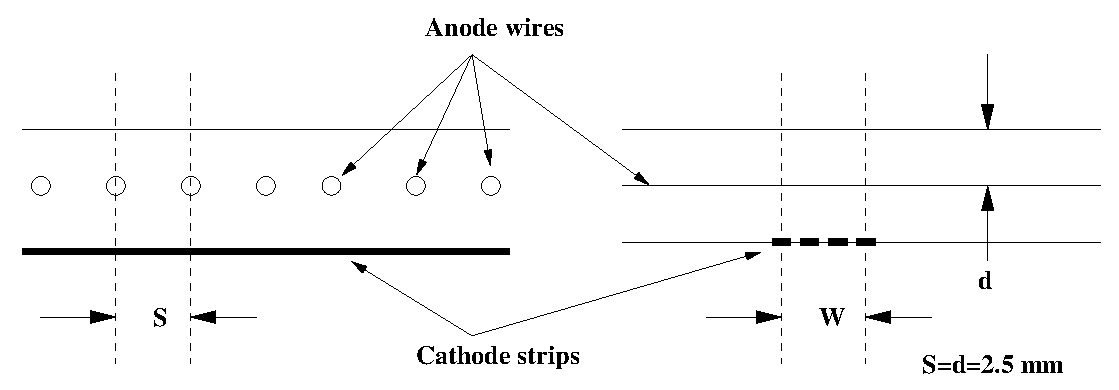
\includegraphics[width=0.85\textwidth, angle=0]{figures/LHC_ATLAS/CSC_structure.eps}
\caption[~Schematic Representation of CSC chambers]{ Schematic Representation of CSC chambers.\cite{ATLAS_JINST} \label{LHC:fig:MDT}}
%\end{center}
\end{figure}

\subsubsection*{Muon Trigger Chambers}

\indent  The ATLAS MS also features a system of fast trigger chambers consisting of three stations of Resistive Plate Chambers (RPC) in the barrel and 4 stations of Thin Gap Chambers (TGC) in the endcap.  The MS triggering system provides triggering coverage up to an $|\eta|$ of 2.4.  The RPCs are placed below and above the middle MDT station and outside the outer MDT barrel station.  The TGC stations are arranged with one station in front of the inner endcap precision tracking wheel and 3 stations split in front and behind the middle endcap MDT wheel.  \\

\indent In Run 2, muon triggers in the endcap also require coincidences in the inner-most layer of the TGC to reduce fake trigger rates due to particles interacting with beam shielding in the forward region. \\

\indent A schematic of the muon trigger system is given in Figure \ref{LHC:fig:MS_trigger}. The trigger searches for fast coincidences between the layers along the expected trajectory of a muon.  Different maximum deviation from the straight infinite momentum path is allowed for triggers with different $\pt$ thresholds. \\

\begin{figure}[h!]
%\begin{center}
\centering
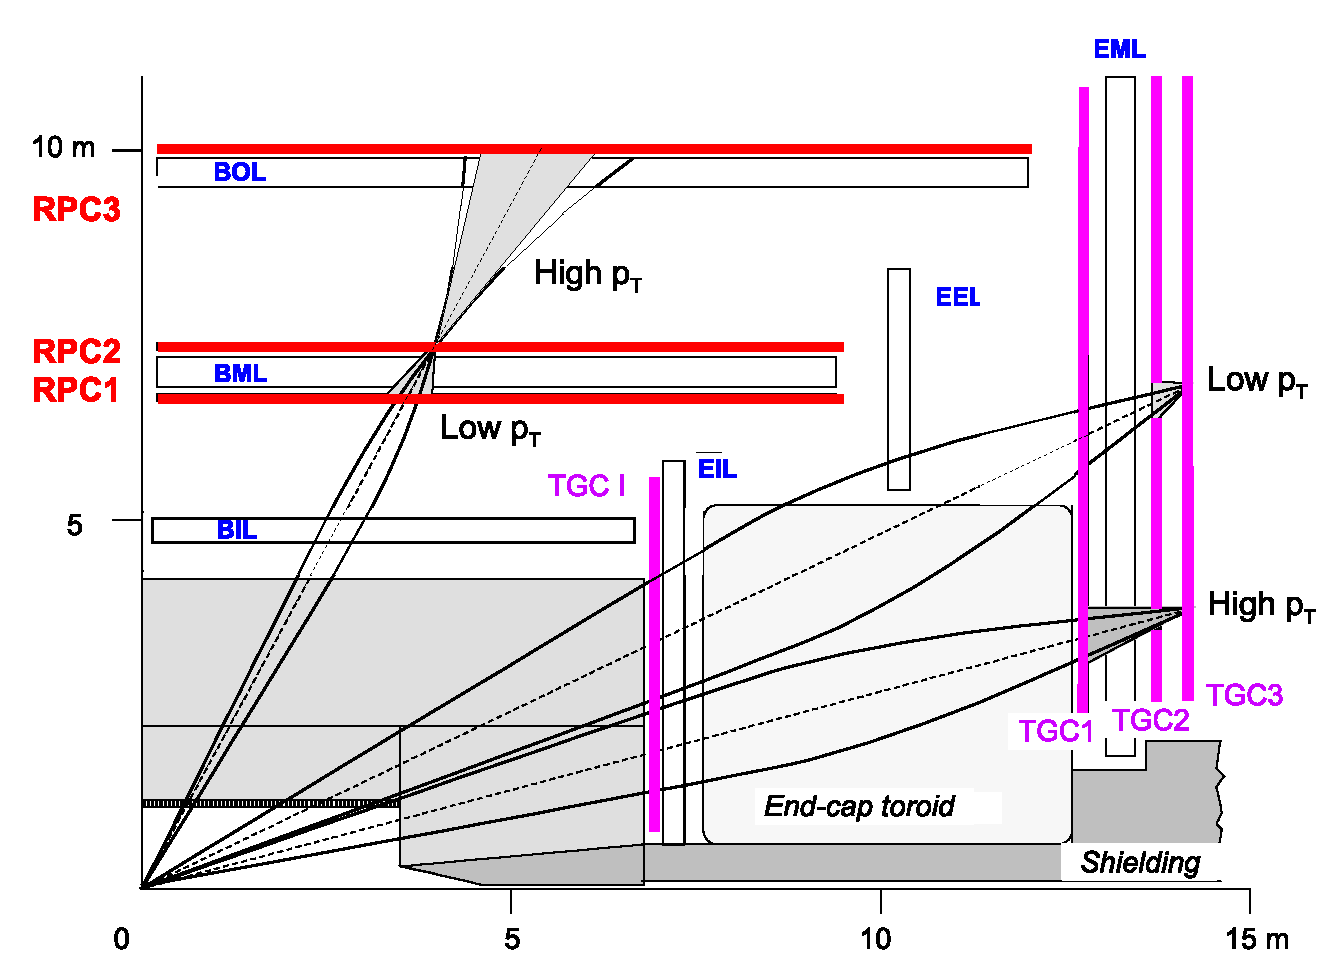
\includegraphics[width=0.75\textwidth, angle=0]{figures/LHC_ATLAS/RPC_TGC_schematics_5.eps}
\caption[~Schematic of the ATLAS muon trigger system]{ Schematic of the ATLAS muon trigger system.  The coincidence windows for muons of different $\pt$ is shown.\cite{ATLAS_JINST} The trigger searches for fast coincidences between the layers along the expected trajectory of a muon.  Different maximum deviation from the straight infinite momentum path is allowed for triggers with different $\pt$ thresholds. High $\pt$ tracks are straighter and lie closer to the infinite momentum straight track than a low $\pt$ track.  \label{LHC:fig:MS_trigger}}
%\end{center}
\end{figure}
